\documentclass[11pt,a4paper]{report} 

% Für doppelseitigen Ausdruck (nur bei > 60 Seiten sinnvoll)
% \usepackage{ifthen}
% \setboolean{@twoside}{true}
% \setboolean{@openright}{true} 

% Deutsch
\usepackage[german]{babel} % deutsch und deutsche Rechtschreibung
\usepackage[utf8]{inputenc} % Unicode Text 
\usepackage[T1]{fontenc} % Umlaute und deutsches Trennen
\usepackage{textcomp} % Euro
\usepackage[hyphens]{url}
% statt immer Ab\-schluss\-ar\-beit zu schreiben
% einfach hier sammeln mit -. 
\hyphenation{Ab-schluss-ar-beit}
% Vorsicht bei Umlauten und Bindestrichen
\hyphenation{Ver-st\"ar-ker-aus-gang}
 % eigene Hyphenations, die für das Dokument gelten
\usepackage{amssymb} % Symbole
\usepackage{emptypage} % Wirklich leer bei leeren Seiten

%% Fonts, je ein kompletter Satz an Optionen

% Times New Roman, gewohnter Font, ok tt und serifenlos
%\usepackage{mathptmx} 
%\usepackage[scaled=.95]{helvet}
%\usepackage{courier}

% Palatino mit guten Fonts für tt und serifenlos
\usepackage{mathpazo} % Palatino, mal was anderes
\usepackage[scaled=.95]{helvet}
\usepackage{courier}

% New Century Schoolbook sieht auch nett aus (macht auch tt und serifenlos)
%\usepackage{newcent}

% Oder default serifenlos mit Helvetica 
% ich kann es nicht mehr sehen ...
%\renewcommand{\familydefault}{\sfdefault}

% ein bisschen eine bessere Verteilung der Buchstaben...
\usepackage{microtype}

% Bilder und Listings
\usepackage{graphicx} % wir wollen Bilder einfügen
\usepackage{subfig} % Teilbilder
\usepackage{wrapfig} % vielleicht doch besser vermeiden
\usepackage{listings} % schöne Quellcode-Listings
% ein paar Einstellungen für akzeptable Listings
\lstset{basicstyle=\ttfamily, columns=[l]flexible, mathescape=true, showstringspaces=false, numbers=left, numberstyle=\tiny}
\lstset{language=python} % und nur schöne Programmiersprachen ;-)
% und eine eigene Umgebung für Listings
\usepackage{float}
\newfloat{listing}{htbp}{scl}[chapter]
\floatname{listing}{Listing}

% Seitenlayout
\usepackage[paper=a4paper,width=14.2cm,left=36mm,height=22cm]{geometry}
\usepackage{setspace}
\linespread{1.15}
\setlength{\parskip}{0.5em}
\setlength{\parindent}{0em} % im Deutschen Einrückung nicht üblich, leider

% Seitenmarkierungen 
\newcommand{\phv}{\fontfamily{phv}\fontseries{m}\fontsize{9}{11}\selectfont}
\usepackage{fancyhdr} % Schickere Header und Footer
\pagestyle{fancy}
\renewcommand{\chaptermark}[1]{\markboth{#1}{}}
%\fancyhead[L]{\phv \leftmark}
\fancyhead[RE,LO]{\phv \nouppercase{\leftmark}}
\fancyhead[LE,RO]{\phv \thepage}
% Unten besser auf alles Verzichten
%\fancyfoot[L]{\textsf{\small \kurztitel}}
\fancyfoot[C]{\ } % keine Seitenzahl unten
%\fancyfoot[R]{\textsf{\small Technische Informatik}}

% Theorem-Umgebungen
\newtheorem{definition}{Definition}[chapter]
\newtheorem{satz}{Satz}[chapter]
\newtheorem{lemma}[satz]{Lemma} % gleicher Zähler wie Satz
\newtheorem{theorem}{Theorem}[chapter]
\newenvironment{beweis}[1][Beweis]{\begin{trivlist}
\item[\hskip \labelsep {\textit{#1 }}]}{\end{trivlist}}
\newcommand{\qed}{\hfill \ensuremath{\square}}

% Quellen teilen
\usepackage{bibtopic} 

% Hochschule Logo, noch nicht perfekt
\usepackage{hsmalogo}

% Spezialpakete
\usepackage{epigraph}
\setlength{\epigraphrule}{0pt} % kein Trennstrich

% damit wir nicht so viel tippen müssen, nur für Demo 
\usepackage{blindtext} 

% Zum Zeigen von Fehlern
\usepackage{soul}
\newcommand*\falsch{\st}

\usepackage{hyperref}
\hypersetup{
    colorlinks=true,
    linkcolor=blue,
    filecolor=magenta,      
    urlcolor=cyan,
    pdftitle={Overleaf Example},
    pdfpagemode=FullScreen,
    }

\newcommand{\tabitem}{~~\llap{\textbullet}~~}

\usepackage{xcolor}
\lstdefinestyle{customcs}{
  keywordstyle=\color{teal},
  identifierstyle=\color{violet},
  stringstyle=\color{orange}
}
 % alle Pakete und Einstellungen

%\bibliography{online}

% Hier anpassen 
\newcommand{\welchethesis}{Bachelor}
% \newcommand{\welchethesis}{Master}
\newcommand{\thesisofwas}{of Science}
\newcommand{\studiengang}{Technische Informatik}
% \newcommand{\studiengang}{Medizintechnik}
\newcommand{\titel}{Smartphones als Sensor- und Aktor}
\newcommand{\kurztitel}{Template Abschlussarbeit}
\newcommand{\autor}{Marius Cerwenetz}
\newcommand{\datum}{08. Juli 2022} % Abgabedatum
\newcommand{\ort}{Mannheim}
\newcommand{\referent}{Prof.\ Dr.\ Peter Barth}
\newcommand{\korreferent}{Prof.\ Dr.\ Jens-Matthias Bohli}

\begin{document}
\begin{titlepage}
  % Kopf der Seite
  \hsmalogo[1] \hfill
  \parbox[b]{60mm}{
    % \textsf würde das Aussehen der ersten Seite ruinieren, 
    % wer will, soll das selbst außen rum machen...
    Fakultät Informationstechnik\\
    Studiengang \studiengang}
  \begin{center}
    % rumfiddeln, damit es für 4 Zeilen gerade noch so geht...
    \rule{1\textwidth}{1pt}\\[-3mm]
    \parbox[t][64mm]{110mm}{% 11 cm für Breite 13, ca. 7 für Höhe 6
      \begin{center}
        \Large{\welchethesis arbeit}\\[2mm]
        {\begin{spacing}{1.13} \huge \bfseries \titel \end{spacing}}
        \vfill
        \Large{\autor} \\[1mm] % keep space to window
        \ 
      \end{center}
    }
    \rule{\textwidth}{1pt}    
    \vfill    
    {\Large Abschlussarbeit} \\[5mm]
    {\large zur Erlangung des akademischen Grades} \\[5mm]
    {\large \welchethesis\ \thesisofwas} \\[5mm]
    \vfill    
    \begin{tabular}{ll} % Mitte der Seite
      Vorgelegt von & \autor \\
      am & \datum \\
      Referent & \referent \\
      Korreferent & \korreferent
    \end{tabular}    
    \vfill
  \end{center}
\end{titlepage}
\cleardoublepage


% Erklärung gemäß der Prüfungsordnung
\thispagestyle{empty}
\subsection*{Schriftliche Versicherung laut Studien- und Prüfungsordnung}

Hiermit erkläre ich, dass ich die vorliegende Arbeit selbstständig verfasst
und keine anderen als die angegebenen Quellen und Hilfsmittel benutzt habe.

\vspace{6em}
\noindent\begin{tabular}{p{0.37\textwidth}p{0.56\textwidth}}
\ort, \datum  & \rule{0.56\textwidth}{0.5pt}\\
              & \makebox[1cm]{\ } \autor
\end{tabular}

\vfill

\cleardoublepage

 % Titelseite, Erklärungen, etc.

\begin{abstract}
Um Programmieraufgaben interaktiv zu gestalten eignen sich Projekte mit Microcontrollern besonders gut.
Smartphones bieten einen vergleichbaren Funktionsumfang und müssen meist nicht zusätzlich beschafft werden.
In dieser Arbeit wurde eine Softwarelösung erstellt, um Smartphonesensoren über eine Programmierumgebung auszulesen und Ausgaben auf dem Smartphone auszuführen.
Hierfür wurde eine Android-Anwendung, eine Kontrollanwendung und eine programiersprachenunabhängige Softwarebibliothek erstellt.

Für die Nutzung der Lösung werden Beispiel-Programmieraufgaben dazugereicht.
Programmierer schreiben Programme auf dem PC, welche auf Änderungen von Smartphonesensorwerten wie beispielsweise Beschleunigungssensoren reagieren und die Ausgabemöglichkeiten des Smartphones nutzen.
\end{abstract}

\tableofcontents

\chapter{Einführung} \label{chap:intro}
Viele Programmierer mühen sich zu Anfang mit der Semantik von Programmiersprachen und grundlegenden algorithmischen Konzepten.
Akademische Übungsaufgaben senken die Lernmotivation und abstrahieren gelerntes.
Projekte mit Microcontrollern dagegen bieten eine praktische, fordernde und spielerische Einstiegsmöglichkeit.
Es werden kleine Projekte realisiert, die durch die Inbezugnahme von Sensoren Programmierer einladen sich an Programmieraufgaben auszuprobieren.
Diese Eigenschaften sind sinnvoll, insbesondere bei Projekten für Programmierer mit wenig Vorwissen wie Schüler oder Erstemester-Studierende.
Gelerntes kann direkt angewandt werden.
Praktische Programmieraufgaben bieten für Programmieranfänger den besten Lerneffekt bei höchster Motivation.\cite{learning_computer_programming}
Die in Microcontroller integrierten Sensoren sind Voraussetzung um physische Eigenschaften in der realen Welt zu messen.
Auf diese Eigenschaften und ihre Änderung kann entsprechend reagiert werden.
Im Programm beschriebene Abläufe definieren Funktion und Verhalten des Microcontrollers bei Änderungen der Sensorwerte.
Geräte erscheinen dann für Nutzer bedienbar.
Während der Entwicklung können Messergebnisse jedoch nicht perfekt vorausbestimmt werden.
Bei anschließenden Tests fällt häufig ein Fehlverhalten auf.
Dann muss das Programm gegebenenfalls angepasst werden, bis das gewünschte Verhalten vorliegt.
Die ständige Weiterentwicklung mindert Ängste vor Änderungen des Codes.
Kontakt schafft Routine und damit ein tieferes Verständnis und Hintergrundwissen für die Problemstellung.

Microcontroller-Projekte benötigen allerdings kostspielige Einstiegs-Kits.
Ein Arduino-Development-Board kostet im Arduino-Shop über 80,00 € \cite{arduino_kit}.
Ein Großteil der Kosten entfällt zwar auf den eigentlichen Microcontroller, ein nicht unmittelbarer Teil jedoch auf Peripherie wie wie Breadboards, Verbindungskabel und Erweiterungsboards.
Sie setzen außerdem gewisses Hintergrundwissen voraus.
Für die erstmalige Verwendung von Breadboards muss beispielsweise bekannt sein, welche Ports wie verbunden sind, welche Konventionen es für Plus- und Minuspole gibt und welche Bauteile für die Benutzung geeignet sind.
Dies stellt ebenfalls eine Einstiegshürde dar, die die eigentliche interaktive Lernerfahrung herauszögert und die Motivation senkt.
Smartphones dienen hier als Alternative.
Aktuelle Smartphones sind mit zahlreichen Sensoren wie Lagesensoren, Gyroskop oder Näherungssensoren ausgestattet.
Sie bieten einen ähnlichen Funktionsumfang wie vergleichbare Microcontroller.
Elektrische Bauteile konventioneller Microcontroller-Sets erlauben einen Fehlgebrauch, der im schlimmsten Fall in der Zerstörung von Komponenten enden kann.
Projekte mit Smartphones reduzieren dieses Risiko dadurch, dass Schaltkreise bereits intern verknüpft und somit von äußerlicher Fehlverwendung geschützt sind.
Ein weiterer Vorteil Smartphones gegebüber Microcontrollern liegt in der Verfügbarkeit.
Weltweit besaßen 2022 5,2 Mrd. Menschen ein Smartphone. \cite{smartphone_users}
Viele Kinder besitzen bereits eins mit 10 Jahren \cite{bitkom_smartphones}.
Da ein Smartphone üblicherweise nicht nur für Programmieraufgaben, sondern auch für den Alltag verwendet wird, sind Smartphones oft bereits in Besitz.
Durch Ihre eingesetzten Sensoren können Sie zuverlässig Umgebungseigenschaften messen.
Neben kabelgebundenen Übertragungsschnittstellen wie USB besteht auch die Möglichkeit sich per W-LAN zu verbinden.
Die Geräte sind zudem batteriebetrieben, was autonome Lösungen ermöglicht.
Eine Einbindung von Smartphones ist in den meisten Prgrammierumgebungen jedoch nicht möglich.
Smartphone-Betriebssystemhersteller bieten keine standardisierten Ausgabemöglichkeiten an.
Moderne Smartphone-Betriebssysteme bauen sich modular aus mobilen Anwendungen auf, so dass das Betriebssystem keine direkten Ausgabemöglichkeiten besitzt.
Visuelle und haptische Ausgaben sind nur über mobile Anwendungen möglich.

Ziel der Arbeit ist es, eine Smartphone-Anwendung für visuelle Ausgaben sowie der Messung und Übertragung von Sensorwerten zu entwickeln.
Außerdem werden Schnittstellen in einer Programmierumgebung geschaffen, die die Interaktionsmöglichkeiten von Smartphones nutzbar macht.
Hierfür stellen Softwarebibliotheken Funktionsaufrufe zur Verfügung um Ausgaben auf dem Smartphone zu tätigen oder Sensorwerte auszulesen.
Das Smartphone reagiert auf die empfangen Anfragen und führt die entsprechenden Kommandos aus.
Zusammengesetzt besteht die Lösung aus einer programmiersprachenunabhängigen Programmierumgebung, einer Kontroll-Anwendung und einer mobilen Anwendung für Android Smartphones.
Für die Verwendung werden angehenden Programmiereren Beispielaufgaben gereicht.
Um die Beispielaufgaben zu bewältigen muss die Lösung auch Benutzungsmöglichkeiten bereitstellen.
Hierdurch werden Anforderungen an Sie gestellt.
Die Aufgaben, Anforderungen und Rahmenbedingungen sind in Kapitel \ref{chap:Experimente} zu finden.
Die drei Komponenten Smartphone-App, Kontrollanwendung und Programmierumgebung und ihr Zusammenspiel werden
in Kapitel \ref{chap:architektur} vorgestellt.
Die dafür benötigten Nachrichtenformate werden in Kapitel \ref{chap:message_formats} gezeigt.
Ihr Zweck wird erklärt und und der Nachrichtenaustausch dort exemplarisch veranschaulicht.
Kapitel \ref{chap:app} behandelt die Funktionsweise und den Aufbau der Android-App im Detail.
Diese tauscht Nachrichten mit der Programmierumgebung aus.
Als Zwischenvermittlung fungiert das zentrale Kontrollprogramm, was in Kapitel \ref{chap:server_software} erklärt wird.
Einbindung, Nutzung, und externe Schnittstellen der Bibliotheken zur Android-App und dem Kontrollprogramm werden in Kapitel \ref{chap:libs} erklärt.
In Kapitel wird \ref{chap:eval} untersucht, ob die vorgegebenen Anforderungen erfüllt wurden.
Dort wird zudem die Verwendung der Lösung anhand einer Beispielaufgabe vorgestellt.
Schwierigkeiten die bei der Entwicklung auftraten werden in Kapitel \ref{chap:fazit} diskutiert.
Erweiterungsmöglichkeiten und Verbesserungen werden diskutiert.

\chapter{Smartphones als Microcontroller-Ersatz} \label{chap:Experimente}
Smartphones sind in sich geschlossene technische Geräte, die neben vordefinierten Verbindungsschnittstellen wie einem USB-Port, WLAN und Bluetooth keine weiteren Schnittstellen bieten um externe Hardware und Schaltungen anzuschließen und fernzusteuern.
Microcontroller-Schaltungen zum Programmierenlernen bieten meistens mehrere Ausgabemöglichkeiten wie LEDs, Lautsprecher oder Piepser.
Smartphones können diese Bausteine nicht anschließen aber virtuell darstellen.
Gewohnte Ausgabeelmente können virtualisiert werden.
Die Funktionen sind außerdem nicht nur von Mehrzweck-Ausgaben, wie LED-Grids begrenzt, die zum Beispiel für die Text- oder Bildanzeige verwendet werden können.
Zweckgebundene Elemente wie Textfelder, Textausgaben oder Bildausgaben in der App können beliebig kombiniert werden.
Darüber hinaus ist die Anordnung der jeweiligen Elemente frei wählbar, so dass das Layout anders als bei Microcontrollern auch im Nachhinein noch geändert werden kann.
Die Ausgabemöglichkeiten können in Kombination mit Sensor-Daten verwendet werden, um kleine Programmieraufgaben zu lösen.
Einige Beispiele werden in diesem Kapitel vorgestellt.
Da diese nicht auf einem Microcontroller, sondern einem Smartphone ausgeführt werden, müssen gewisse Rahmenbedingungen erfüllt sein, wie beispielsweise geringe Latenzen in der Sensordatenübertragung.
\section{Beispielprogrammieraufgaben}\label{sec:activities}
Praxisnahe Programmieraufgaben mit interessanten Aufgabestellungen motivieren Softwareentwickler.
In den Aufgaben interaktiv auf die Änderung physikalischer Eigenschaften gewartet und reagiert.
Die Liste der Aufgaben ist in Tabelle \ref{tab:excercises} zu finden.
In ihr ist zu finden, welche Aufgabe welche Sensordaten benötigt werden und welche Ausgabemöglichkeiten genutzt werden sollen
Die Angabe des Schwierigkeitsgrads unterstützt Anfänger bei der Auswahl um die Motivation zu erhöhen.
Er ist in drei Größen gegliedert:
Einfach (+), Mittel(++) und Schwer (+++).
\begin{table}[htbp]
  \centering
  \begin{tabular}{|l|c|p{2cm}|c|}
      \hline
      \textbf{Name der Aufgabe} & \textbf{Benötigte Sensoren} & \textbf{Verwendete Ausgaben} & \textbf{Schwierigkeitsgrad} \\
      \hline
      Disco & - & Led & + \\
      \hline
      Würfeln & Lagesensor & Textfeld &+ \\
      \hline
      Diebstahl-Alarm & Näherungssensor & Textfeld, Led, Vibration & ++ \\
      \hline
      Klatsch-Zähler & Mikrofon & Textfeld & ++ \\
      \hline
      Dreh-Zähler & lagesensor & Textfeld & +++ \\
      \hline
  \end{tabular}
  \caption{Beispielprogrammieraufgaben}
  \label{tab:excercises}
\end{table}

In der Aufgabe \textit{Disco} soll eine virtuelle LED alle 500 ms von der Farbe grün auf die Farbe rot wechseln.
Die Aufgabe benötigt keine Sensoren, da die LED nicht auf eine Eingabe seitens des Programmierers oder sonstigen Messwert-Änderungen warten soll.
Der Schwierigkeitsgrad ist als einfach eingestuft, da hier weder Sensoren benötigt werden, noch sonstige Abhängigkeiten die auf Sensormesswerte beruhen innerhalb des Codes zu berücksichtigen sind.

In der Aufgabe \textit{Würfeln} soll erkannt werden, ob ein Device geschüttelt wurde.
Verwendet wird dabei der Lagesensor, der Beschleunigungen misst.
Wird ein Schütteln erkannt soll auf dem PC eine Zufallszahl generiert werden, welche dann auf dem Device in einem Textfeld ausgegeben wird.
Die Schwierigkeit wird ebenfalls auf einfach eingeschätzt, da lediglich ein Sensor und eine Ausgabe verwendet wird.

In der Aufgabe \textit{Diebstahl-Alarm} soll überprüft werden, ob sich jemand dem Device genähert hat um es zu greifen.
Benötigt wird dafür der Näherungssensor.
Misst er eine Annäherung, soll ein alarmierender Text im Textfeld auf dem Smartphone ausgegeben werden.
Ebenfalls benötigt wird die Vibrationsfunktion als haptisches Feedback.
Bei einer Näherungs-Detektion soll es fünf mal vibrieren.
Außerdem soll die LED die Farbe wechseln, so wie in der Aufgabe \textit{Disco}.
Der Schwierigkeitsgrad der Aufgabe ist als \textit{Mittel} eingestuft, da die Zeitdauer der Vibration länger sein soll als die Pausen zwischen dem Farbwechsel der LED.
Entfernt sich die Person muss der Alarm-Zustand verlassen werden können.
Alle Ausgaben werden auf ihren initialwert zurückgesetzt.

Bei der Aufgabenstellung \textit{Klatsch-Zähler} muss für einen definierten Zeitraum die Anzahl der Händeklatscher gemessen werden.
Programmierer klatschen vor dem Device in die Hände.
Die Anzahl der Klatscher wird gemessen und auf dem Display des Smartphones ausgegeben.
Verwendet wird dafür lediglich das Mikrofon zur Eingabe und das Textfeld zur Ausgabe.
Die Schwierigkeit ist auf \textit{Mittel} angesetzt, da Klatscher unterschidliche Intensitäten haben können.
Programmierer müssen also ausprobieren, wann es sich wirklich um ein Händeklatschen handelt und wann nur Hintergrundgeräusche zu hören sind.

Bei der letzen Aufgabe \textit{Drehzähler} soll der Programmierer das Device innerhalb eines eigenen definierten Zeitraums drehen und anhand der zurückgegeben Werte die Anzahl der Drehungen ermitteln.
Diese soll anschließend im Textfeld auf dem Device ausgegeben werden.
Zur Verwenung kommen hier ebenfalls der Lagesensor als Sensoreingabe und das Textfeld als Ausgabe.
Die Aufgabe ist als \textit{Schwer} bewertet, da hier Wiederholungen in einer Werteabfolge erkannt werden müssen.
Diese sind jedoch nicht immer exakt gleich.
So muss auch ausprobiert werden, wie sich eine Umdrehung in den Messwerten äußert und wie Drehungen optimal erkannt werden können.

\section{Anforderungen}\label{sec:anforderungen}
Geringe Latenzen sind bei der Sensordatenübermittlung nötig, damit Programme bei Messwertänderungen schnell reagieren könnnen.
Damit dies möglich ist müssen die Aufgabenbereiche der Lösung seperiert werden.
Die Komponenten müssen über effiziente Protokolle kommunizieren.
Funktionen die aufgerufen werden um Sensormessdaten zu erhalten müssen ihre Rückgabewerte simpel gestalten.
Serialisierte Formate erfordern zusätzliches Hintergrundwissen.
Um auf die Ergebnisse zurückgreifen zu können müssten weitere Bibliotheken zum Parsen eingesetzt werden.
Das erschwert die Umsetzung der Aufgaben.
Damit das Programm entsprechend schnell auf geänderte Sensordaten reagieren kann, müssen Sie jederzeit angefragt werden können.
So können Experimente eher begriffen werden, da Auswirkungen in der Realität unmittelbar Auswirkungen auf das entwickelte Programm haben.
Idealerweise liegen Sie zum Zeitpunkt der Anfrage bereits vor.
Sensor-Messungen sollten nicht auf eine Anfrage hin gestartet, sondern vorher begonnen werden.
So werden die Latenzzeiten minimiert.
Weiterhin berücksichtigt wird, dass die Sensorwerte einen Transportweg durchlaufen.
Dieser beschreibt die Strecke zwischen Smartphone und Programmierumgebung.
Übertragungsszeiten können je nach Mobilfunk- bzw WLAN Standard, Umwelteinflüssen und Geräteanzahl im Medium variieren.
Die Round-Trip-Time (RTT) dient bei Wireless-Verbindungen als Indikator für Latenzen.
Sie beschreibt die Zeit des Hin- und Rückweges eines Gerätes zu einem Host.
Bei Funk-Verbindungen wie WLAN fällt Sie höher aus als bei kabelgebundenen Medien.
Während Sie bei Standards wie WLAN 802.11b ca. 10 ms beträgt kann Sie bei UMTS auf 300 ms bis 400 ms ansteigen.\cite{network_latencies}
Um diese Latenzen zu verringern müssen Sensorwerte zwischengespeichert werden um einen Puffer aufzubauen auf den in Fällen erhöhter Latenz zugegriffen werden kann.
Dies bedeutet jedoch auch, dass das Smartphone kontinuierlich in periodischen Abständen Sensorwerte senden muss, damit der Puffer gefüllt ist.
Liegen die Daten vor, kann der vom Programmierer entwickelte Algorithmus Ausgaben auf dem Smartphone auslösen.
Ausgabe-Kommandos sind zwar ebenfalls von Latenzen betroffen, haben allerdings keine direkte Auswirkung auf die Entscheidungsstruktur eines Programms.
Sollten Rückgabewerte trotzdem nötig sein und anfallen, ändern Sie sich nicht sehr häufig.
Auf Sie muss seltener reagiert werden.
Der Zweck von Ausgaben mit Rückgabewert besteht in einer Ausführungsmeldung, anstatt einer Meldung von Messergebnissen von denen der weitere Programmablauf abhängt.
Es kann zum Beispiel überprüft werden, ob die Änderungen an den Ausgabemöglichkeiten tasächlich stattgefunden haben.

Neben den kommunikativen Anforderungen muss die Smartphone-App auch Ausgabemöglichkeiten bereitstellen.
Es muss eine signal LED geben, deren Farbe gewechselt werden kann um Änderungen zu signalisieren.
Ein Textfeld muss alphanumerische Zeichen ausgeben können, um sowohl Zahlenwerte, als auch kurze Texte darzustellen.
Die Länge ist jedoch beschränkt, da nur einzelne Werte oder Wörter ausgegeben werden, keine Textabsätze.
Die Vibrationsausgabe ist eine haptische Ausgabe, keine Optische.
Für diese muss eine Zeitdauer konfigurierbar sein um Vibrationsmuster konfigurieren zu können.
\chapter{Architektur} \label{chap:architektur}
Insgesamt besteht die Lösung aus einer Programmierumgebung, einem Kontrollprogramm zur Nachrichtenkoordinierung und einer mobilen Android-Anwendung für die Sensordatenerhebung und für die Anzeige der Ausgaben.
Der Aufbau ist in Abbildung \ref{fig:design} dargestellt.
\begin{figure}[htbp]
\centering
% 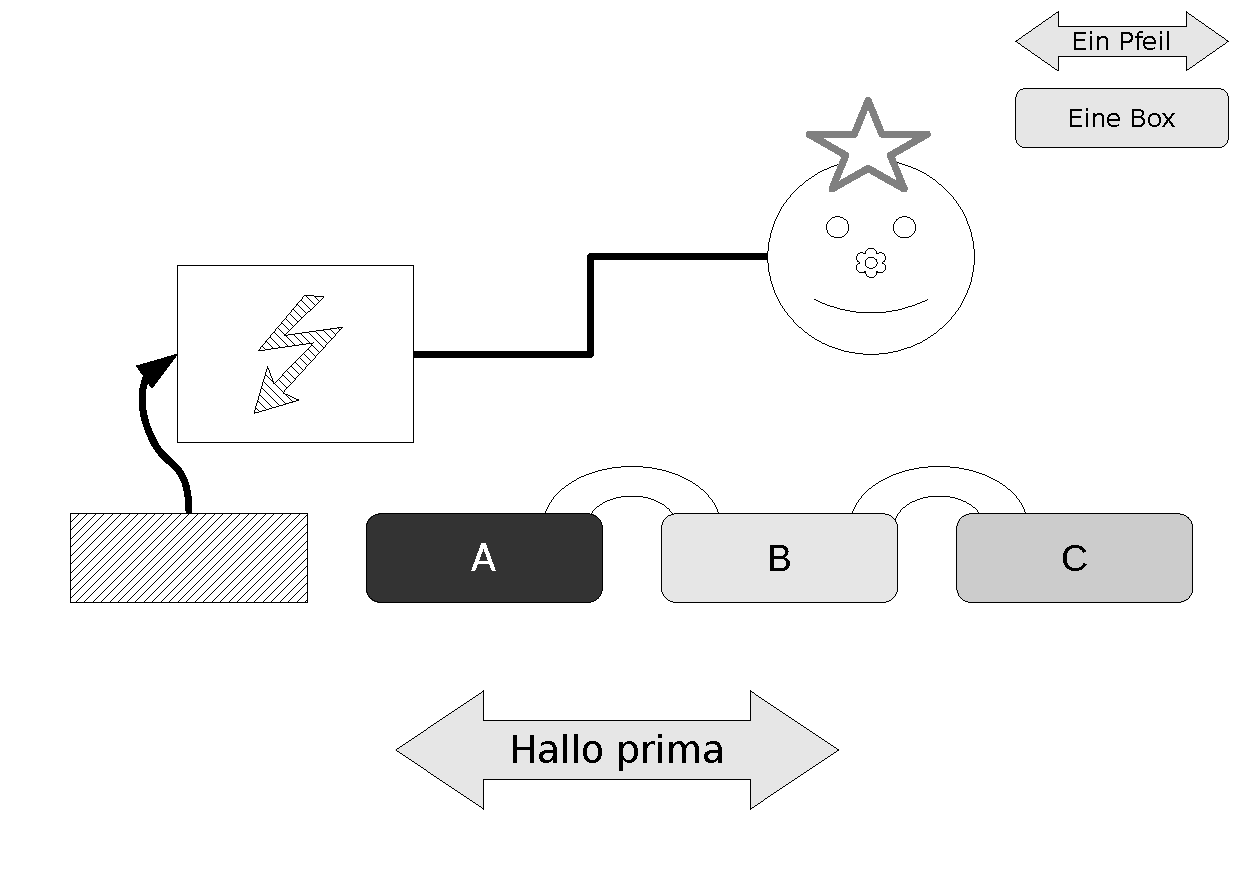
\includegraphics[width=.9\textwidth]{zeichnung.eps}
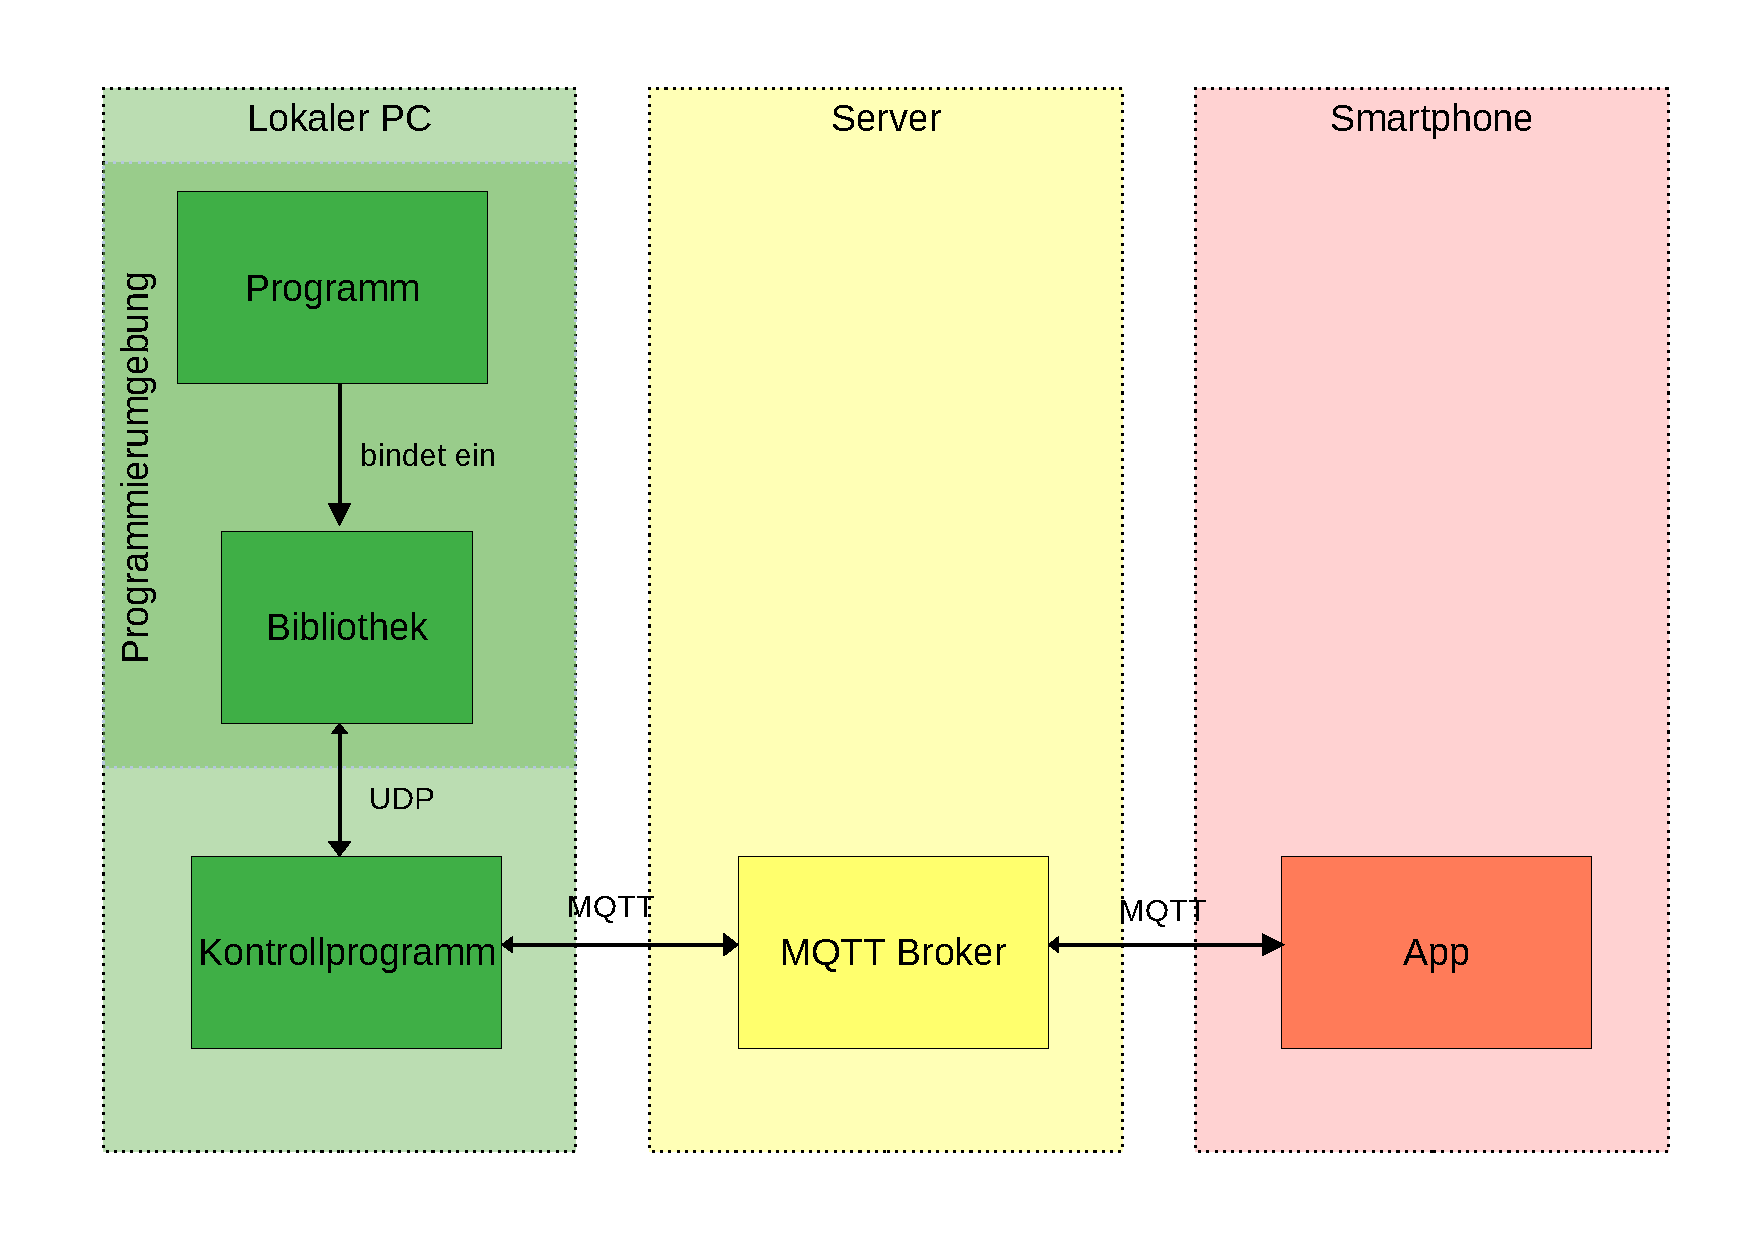
\includegraphics[width=\textwidth]{images/framework.pdf}
\caption{System-Aufbau}
\label{fig:design}
\end{figure}
Die Programmierumgebung besteht aus einer programmiersprachenunabhänigen Bibliothek und dem vom Entwickler geschriebenen Programm.
Der Entwickler kann die Funktionalität der Lösung nach Einbindung der Bibliothek nutzen
Neben der Programmierumgebung läuft auf dem lokalen PC auch das Kontrollprogramm.
Dieses ist für die Koordinierung des Nachrichtenaustauschs zwischen der Android-App und der Programmierumgebung zuständig.
Startet ein Entwickler einen Aufruf der Bibliothek, kommuniziert diese ihn per UDP dem Kontrollprogramm.
Das Kontrollprogramm kommunziert dann weiter über MQTT mit dem Smartphone.
MQTT ist ein auf TCP basierendens Client-Server-Protokoll.
Durch einen 2 Byte großen Header und maximalen Payload-Größe von 260 MB ist es leichtgewichtig und gleichzeitig flexibel.
Nachrichten werden an einen MQTT Broker gesendet, der die Nachrichten dann an alle Clients weiterreicht die das Topic auf dem die Nachricht gesendet wurde abboniert haben.
Die UDP-Kommunikation zwischen Bibliothek und Kontrollprogramm verläuft auf dem lokalen PC über ein Loopback-Interface.
Das Kontrollprogramm erfüllt drei Aufgaben: Die Beantwortung von Sensoranfragen der Bibliothek, dem Zwischenspeichern von Sensorwerten in einem Pufferspeicher und dem Weiterleiten von Ausgabe-Kommandos auf das Smartphone.
Bei Sensoranfragen werden von der Bibliothek aus an die Kontrollanwendung gesendet.
Dieses beantwortet Sie mit dem aktuell vorliegenden Sensorwert.
Die Sensorwerte werden fortlaufend durch das Smartphone aktualisiert.
Es sendet fortwährend aktuelle Sensordaten an das Kontrollprogramm.
Dieses nimmt Sie entgegen und sichert Sie in einem internen Puffer.
Ausgabe-Anfragen für das Smartphone werden ebenfalls über das Kontrollprogramm an das Smartphone per MQTT gesendet.
Die Smartphone-Anwendung beginnt sobald Sie startet mit der Erhebung der Sensordaten, welche sie anschließend an die Kontrollanwendung sendet.
Daneben reagiert Sie auf Ausgabeanfragen von der Bibliothek, welche bei Eingang ausführt werden.


\chapter{Nachrichtenformate}\label{chap:message_formats}
Ein einheitliches Kommunikationsformat ist für den Nachrichtenaustausch unabdingbar.
Der zur Übermittlung ausgearbeitete Standard definiert die Nachrichten in einem Klartextformat.
Als Darstellungsform wird JSON verwendet.
Die in einer Datei gespeicherten Nachrichten-Vorlagen werden in der Bibliothek, dem Kontrollprogramm und in der Smartphone-App eingelesen
So sind die Nachrichten in jeder Komponente gleich.
Es gibt unterschiedliche Nachrichtentypen für verschiedene Zwecke.
Diese sind in Tabelle \ref{tab:message_types} aufgeführt.
Um besser nachvollziehen zu können welche Kommunikationspartner welche Nachrichten austauschen, sind außerdem Quelle und Ziel und das verwendete Netzwerkprotokoll angegeben.
\begin{table}[htbp]
  \centering
  \begin{tabular}{|l|p{30mm}|c|c|}
      \hline
      \textbf{Nachrichtentyp} & \textbf{Quelle} & \textbf{Ziel} & \textbf{Netzwerkprotokoll}\\
      \hline
		sensor\_request & Bibliothek & Kontrollprogramm & UDP\\
       \hline
       sensor\_response & Kontrollprogramm & Bibliothek & UDP\\
       \hline
		update\_request & Smartphone & Kontrollprogramm & MQTT\\
       \hline
		rpc\_request & Bibliothek, Kontrollprogramm & Smartphone & UDP/MQTT\\
       \hline
		rpc\_response & Smartphone, Kontrollprogramm & Bibliothek & UDP/MQTT\\ 
       \hline
  \end{tabular}
  \caption{Nachrichten-Typen}
  \label{tab:message_types}
\end{table}

\textit{Sensor\_request}s kommen zum Einsatz, wenn Programmierer einen Sensorwert abfragen.
Dann wird die Nachricht von der Bibliothek an das Kontrollprogramm gesendet.
Dieses hat vom Smartphone übermittelte Sensorwerte zwischengespeichert.
Nach Eingang ermittelt das Kontrollprogramm den gewünschten Sensorwert.
Die Angabe des gewünschten Sensors wird im Feld \texttt{sensor\_type} beschrieben.
Ist er in der gespeicherten Datenstruktur zu finden, wird er in einer neuen Nachricht im Nachrichtenformat \textit{sensor\_response} zurückgesendet.
Der gespeicherte Wert ist im Feld \texttt{sensor\_value} zu finden.
Die Antwort wird von der Bibliothek angenommen und anschließend an das Programm des Entwicklers zurückgegeben, das den Sensortwert ursprünglich forderte.
Sensor-Abfragen laufen blockierend ab.
Das bedeutet, dass jede Sensor-Wert-Anfrage immer erst eine Rückgabe erhalten muss, bevor die nächste Sensor-Wert-Anfrage gestartet werden kann.
Es ist unmöglich, dass die Kontrollanwendung zwei Sensor-Wert-Anfrage gleichzeitig erhält und die Antworten in umgekehrter Reihenfolge zurücksendet, was eine Vertauschung der Sensorwerte bedeutete.
Durch  Angabe des ursprünglich geforderten Sensor-Typs in der Antwort könnte dies verhindert werden, ist allerdings nicht nötig.
Sensorwerte müssen kontinuierlich vom Smartphone aktualisiert werden, damit das Kontrollprogramm immer den aktuellste Wert zurückliefern kann.
Die Android-App sendet daher in periodischen Abständen Nachrichten des typs \textit{update\_request} an das Kontrollprogramm.
Sie kann für jede Sensor-Art verwendet werden.
Übermittelt wird sowohl der Sensor-Typ, als auch der gemessene Sensor-Wert.
Die Kontrollanwendung kann den den Wert über den Typ zuordnen und in den internen Datenpuffer eintragen.
Der gesamte Ablauf für Sensoranfragen ist in Abbildung \ref{fig:message_flow_requests} dargestellt.
\begin{figure}[htbp]
\centering
% 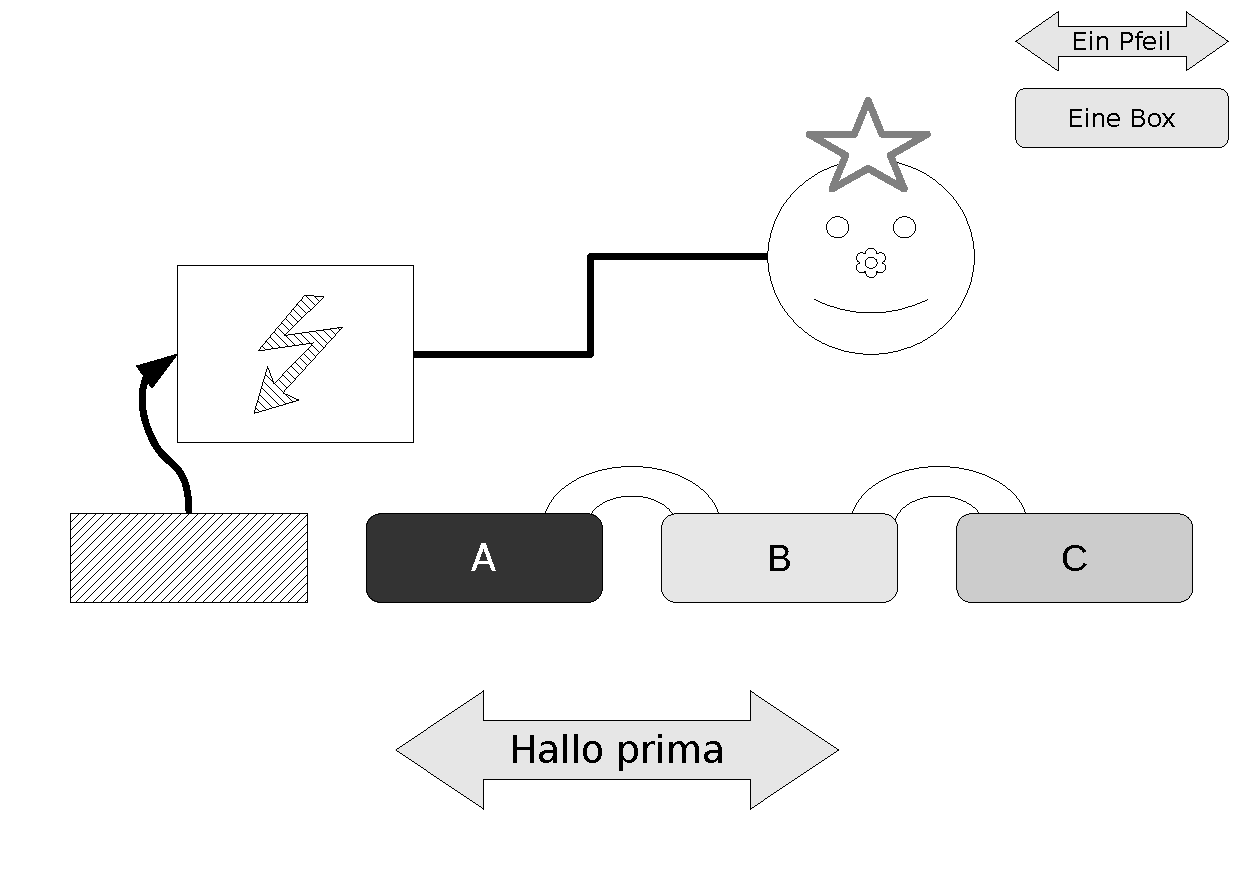
\includegraphics[width=.9\textwidth]{zeichnung.eps}
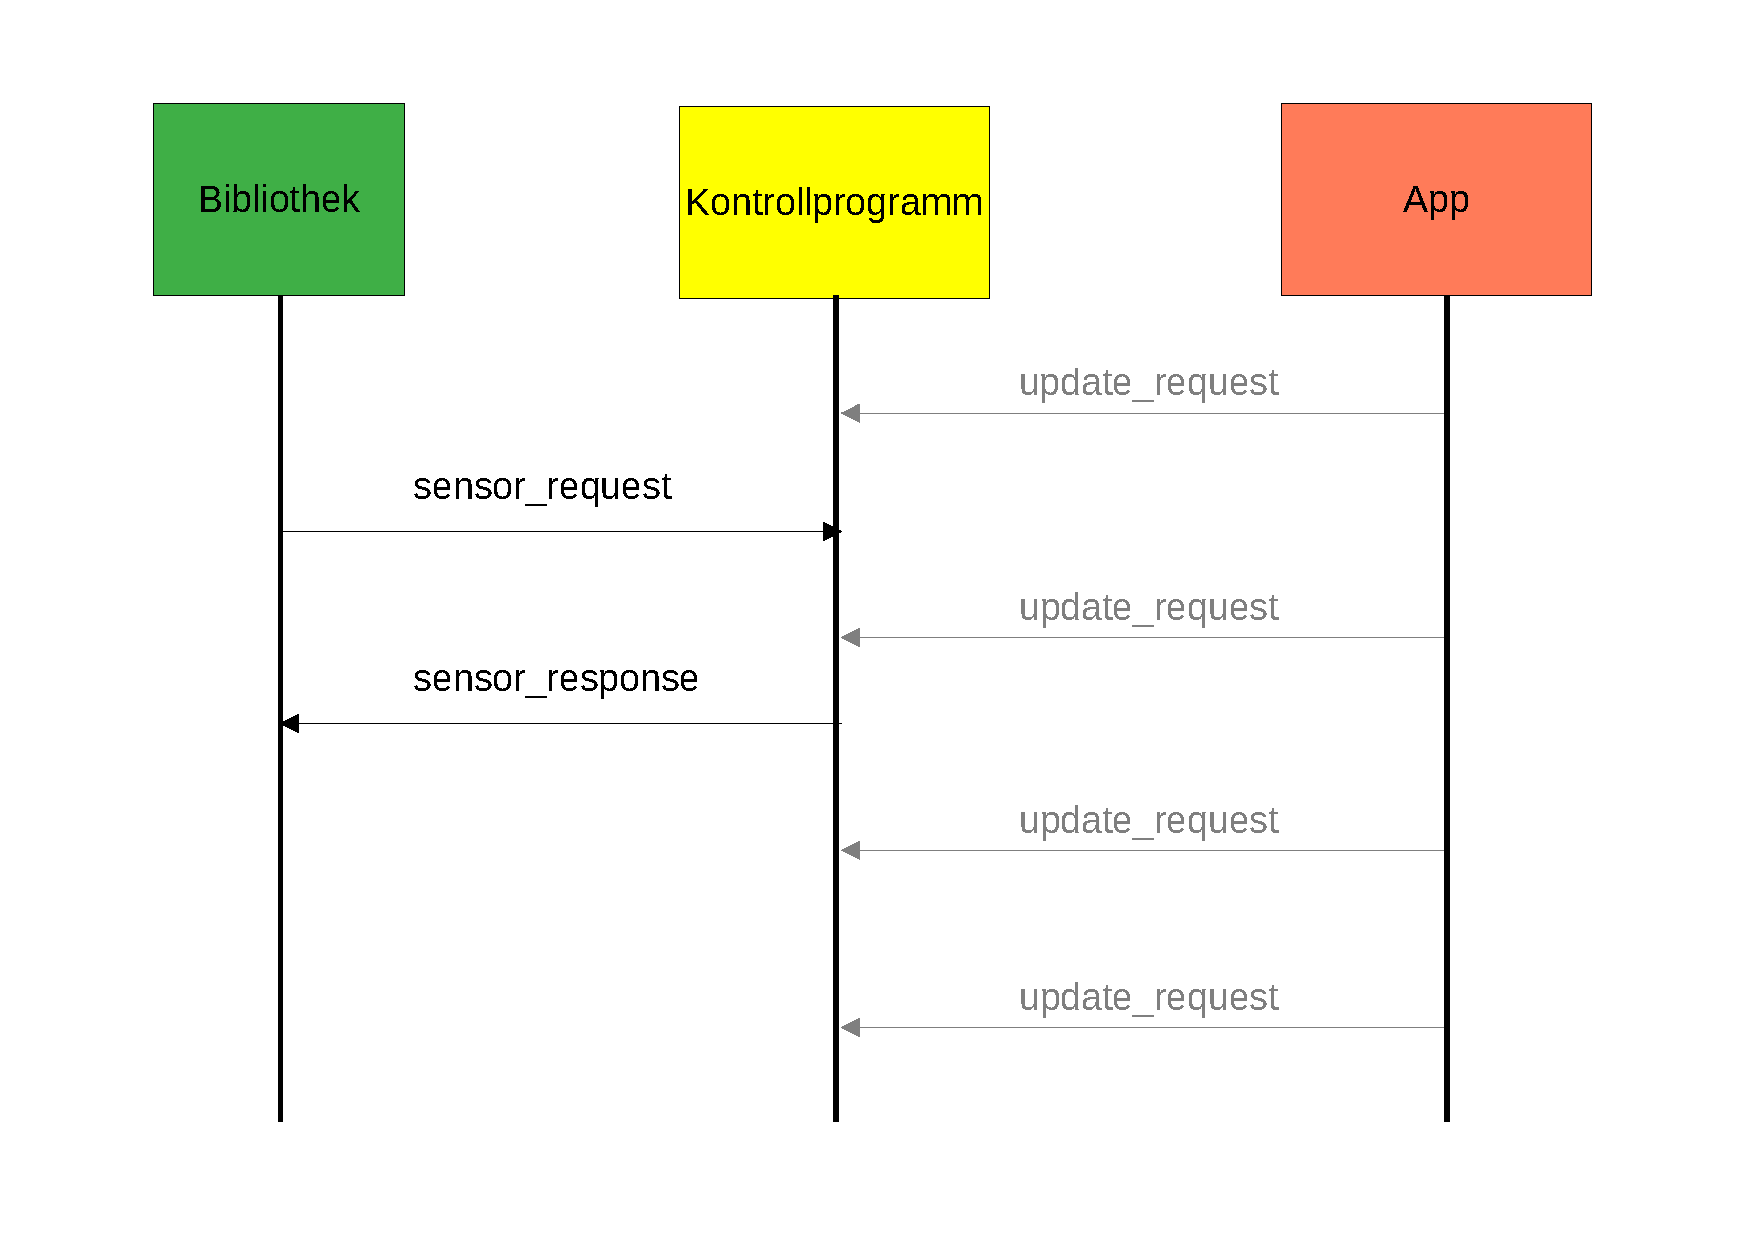
\includegraphics[width=.9\textwidth]{images/message_flow_sensor.pdf}
\caption{Nachrichtenablauf der Sensordatenübermittlung}
\label{fig:message_flow_requests}
\end{figure}
Zu sehen sind die drei Komponenten Bibliothek, Kontrollprogramm und App auf dem Smartphone.
Die Bibliothek sendet sensor\_requests per UDP an das Kontrollprogramm.
Dieses antwortet über UDP mit einer sensor\_response.
Währenddessen sendet die App auf dem Smartphone kontinuierlich update\_requests per MQTT um der Kontrollanwendung neue Messergebnisse mitzuteilen.

Neben den Sensordaten betreffenden Nachrichten existieren auch Ausgabe-Kommandos um Ausgaben in der Smartphone-App umzusetzen.
Es wird unterschieden Ausgaben mit und ohne Rückgabewert.
Für erstere gibt es den Nachrichtentyp \textit{rpc\_request}.
RPC steht für Remote Procedure Call und bezeichnet Clientseitige Funktionsaufrufe, die auf einem Server ausgeführt werden.
Die Bezeichnung entspricht nicht dem Konzept, da die die Smartphone-App in diesem Fall die Rolle des Servers einnehmen würde.
Die Voraussetzung einer Client-Server-Anwendung ist dadurch nicht gegeben.
Kommunikationspartner tauschen auf gleicher Ebene Daten aus.
Die Bezeichnung wurde unter dem Fokus auf der entfernten Ausführung einer Funktion gewählt.
Der Nachrichtentyp enthält die Felder \texttt{command} und \texttt{value}.
Ersters spezifiziert das Ausgabe-Kommando, das Zweite die Größe des Parameters für das Ausgabekommando.
Es ist fast immer befüllt.
Vereinzelt gibt es jedoch auch Kommandos die keinen Parameter benötigen.
Dann bleibt dieses Feld leer.
Die Nachricht wird von der Bibliothek per UDP an die Kontrollanwendung und von dort aus per MQTT an das Smartphone gesendet.
Die Smartphone-App nimmt die Anfrage an und führt die Ausgabe aus.
Manche Kommandos erheben zusätzlich einen Rückgabewert.
Damit dieser vom Smartphone zurück an die Bibliothek gesendet werden kann, gibt es das Nachrichtenformat \textit{rpc\_response}.
Dieses wird erst per MQTT an das Kontrollprogramm und von dort aus per UDP an die Bibliothek gesendet.
Wie bei sensor\_responses können sich die Antworten nicht gegenseitig überholen, was die Übertragung des zugrundeliegenden Ausgabe-Kommandos überflüssig macht.
Nur der ermittelte Wert des Kommandos ist relevant und wird in der Nachricht übermittelt.
Der Nachrichtenablauf wird in Abbildung \ref{fig:message_flow_rpc} zusammengefasst.
\begin{figure}[htbp]
\centering
% 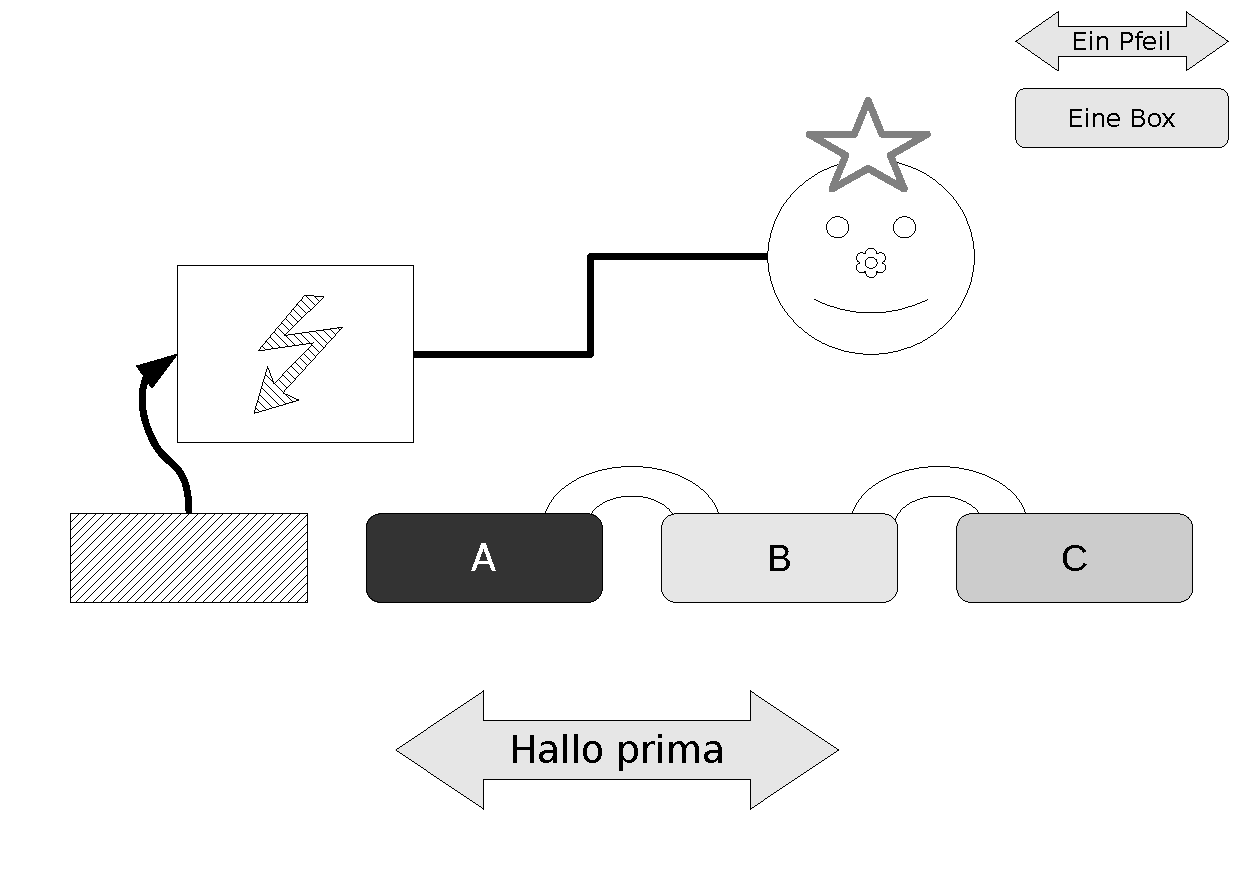
\includegraphics[width=.9\textwidth]{zeichnung.eps}
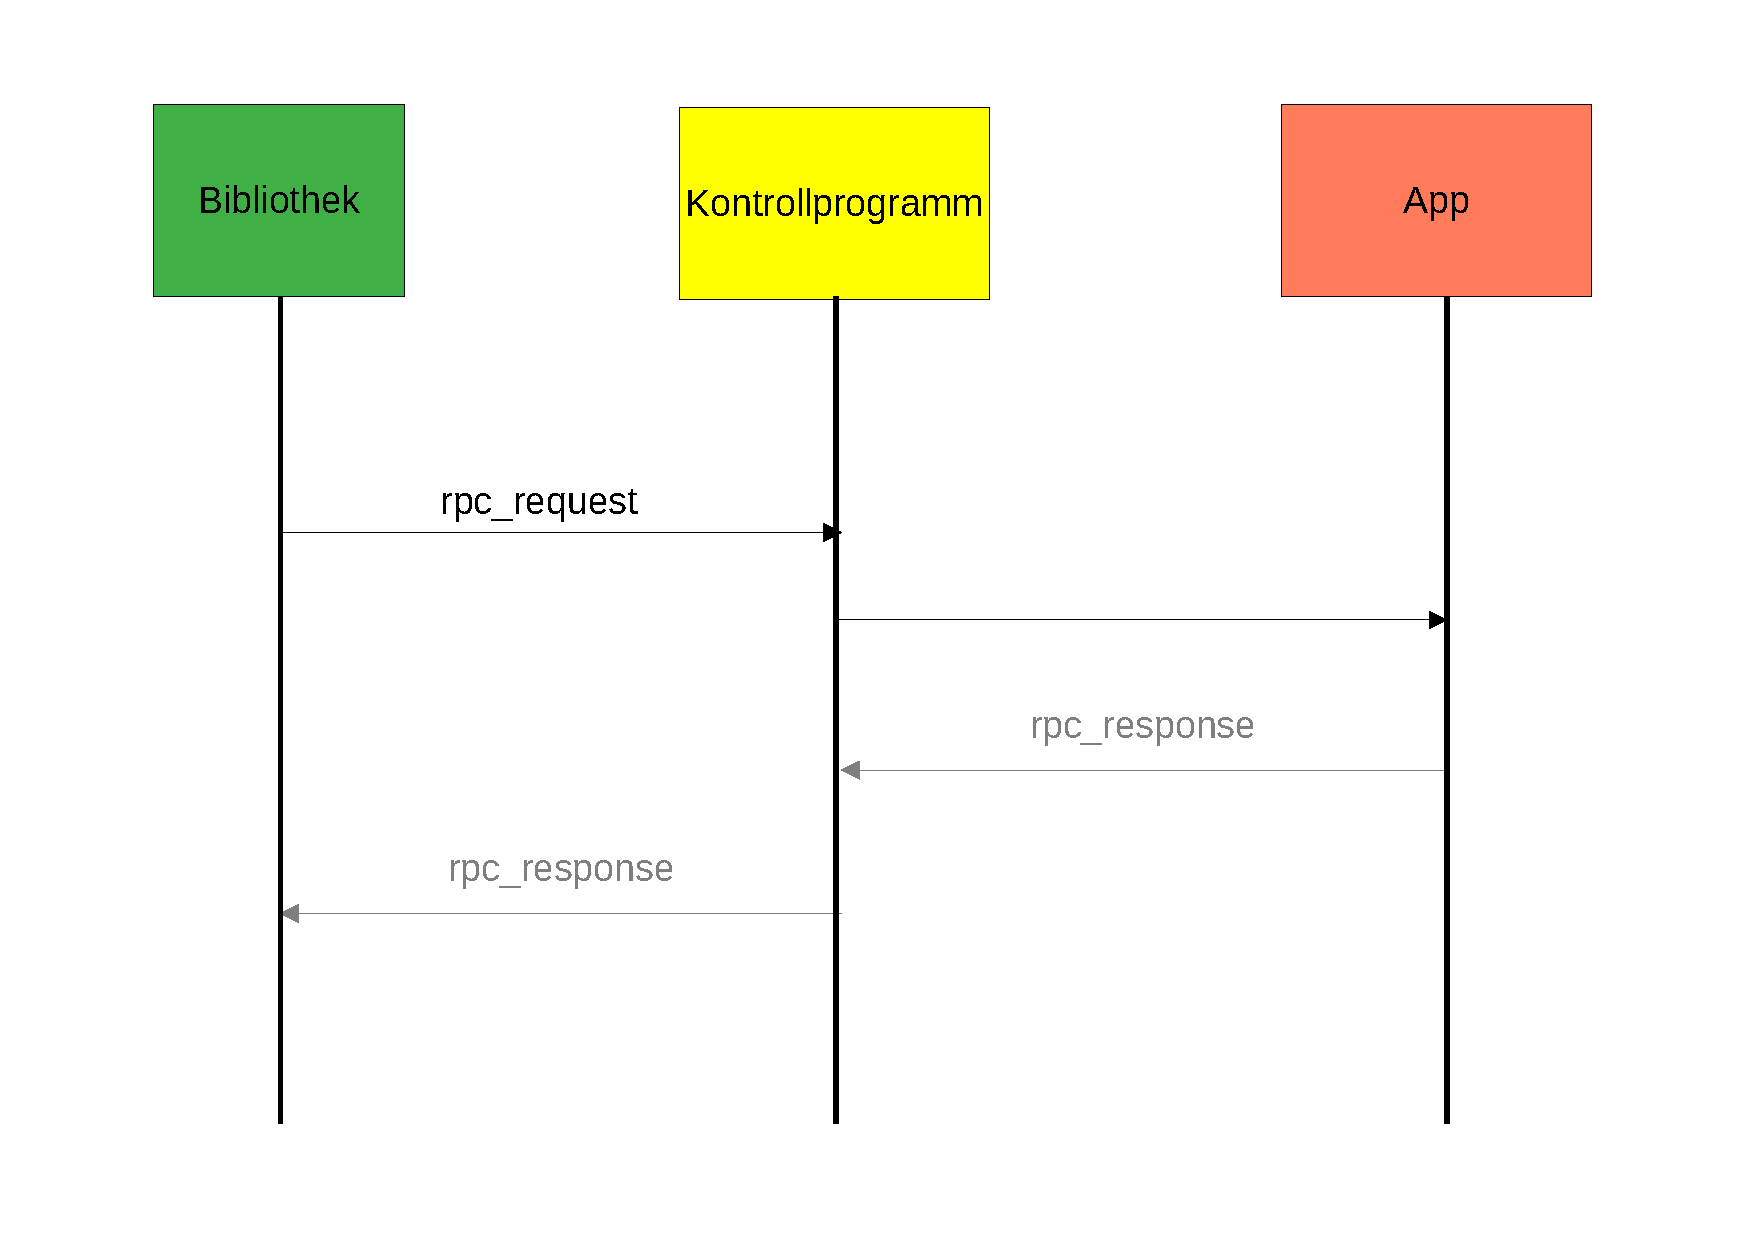
\includegraphics[width=.9\textwidth]{images/message_flow_rpc.pdf}
\caption{Nachrichtenablauf der RPC-Anfragen}
\label{fig:message_flow_rpc}
\end{figure}
Zu sehen sind die drei Komponenten Bibliothek, Kontrollprogramm und Android-App.
Die Bibliothek sendet rpc\_requests per UDP an das Kontrollprogramm.
Dieses leitet die Nachricht per MQTT direkt weiter an die App.
Dort wird das gewünschte Kommando ausgeführt.
Fällt ein Rückgabewert an, wird eine rpc\_response generiert und vom Smartphone per MQTT zurück an die Kontrollanwendung gesendet.
Diese leitet die Nachricht dann per UDP weiter an die Bibliothek.

\chapter{Android Anwendung}\label{chap:app}
Die Android-Anwendung ist eine der drei zentralen Bestandteile des Frameworks.
Sie dient dazu Sensormessprozesse zu starten, Sensordaten zu übermitteln und Ausgabe-Kommandos auszuführen.
Für diese bietet Sie unterschiedliche UI-Elemente in einer Activity, der RootActivity ein.
Sie besteht aus einer Signal-Led, einem Textfeld und zwei Buttons.
Neben UI Elementen gibt es zusätzlich noch eine Vibrationsausgabe. 
Die Anwendung misst Sensorwerte und sendet Sie an die Kontrollanwendung.
Messungen werden über SensorEventListener realisiert.
Sie starten Messvorgänge und ermitteln periodischen Zeitabständen den aktuell vorliegenden Messwert.
Jedes Messergebnis wird anschließend per MQTT an die Kontrollanwendung gesendet.
Versandt werden die Sensorwerte über den MQTT-Service, einem App-Service, der im Hintergrund ausgeführt wird.
Dieser reagiert ebenfalls auf eingehende Anfragen um Ausgaben auf dem Smartphone auszulösen.
Gibt die Ausgabe einen Rückgabewert zurück, werden rpc\_response-Nachrichten an die Kontrollanwendung und schlussendlich an die Bibliothek gesendet.

\section{Funktionsablauf}
Die Erhebung der Messwerte erfolgt zum Start der Anwendung.
Ein Ablaufplan ist in Abbildung \ref{fig:app_flow} zu sehen.
\begin{figure}[htbp]
  \centering
  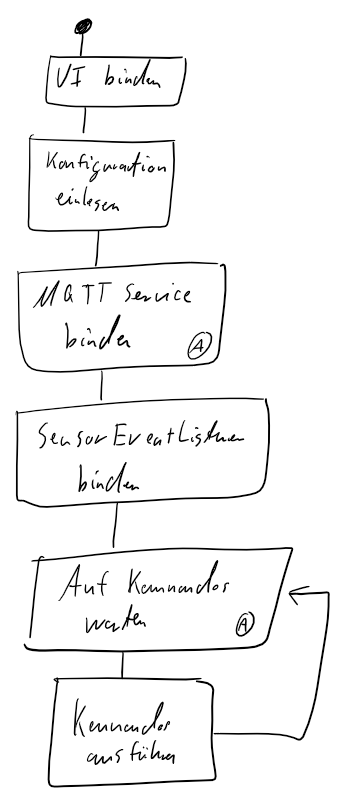
\includegraphics[width=0.8\textwidth]{images/app_ablauf}
  \caption{Ablaufdiagramm Android Anwendung}
  \label{fig:app_flow}
\end{figure}
In der Root-Activity werden zuerst alle UI-Elemente eingebunden um Sie über Kommandos zu manipulieren.
Anschließend werden Konfigurationsdaten eingelesen.
Insgesamt gibt es zwei Konfigurationsdateien: config.json und protocol.json.
In Ersterem ist zum Beispiel der Hostname des MQTT-Brokers, der Port oder das Topic definiert.
Diese Daten sind für die Übermittlung der Nachrichten per MQTT wichtig.
In protocol.json wird die Form der für das Smartphone relevanten Nachrichtenformate update\_request und rpc\_response definiert.
Außerden sind dort die unterstützten Sensoren und Ausgabekommandos beschrieben.
Relevant werden diese bei der Entscheidungsfindung bei Eingang eines rpc\_requests, wenn determiniert werden muss welche Aktion die Nachricht beeinhaltet.
\\
Nach dem Einlesen der Konfigurationen wird der zur Kommunikation verwendete MQTT Service eingebunden.
Dies geschieht asynchron.
Über eine ServiceConnection wird beim erfolgreichen einbinden über eine Callback-Methode der weitere Verlauf definiert.
Die Root-Activity speichert dann die Referenz auf den Service und der Service die Referenz auf die Root-Activity.
Grund für dieses gegenseitige Einbinden ist, dass Nachrichten im MQTT Service in einem seperaten Thread behandelt werden.
Bei RPC-Requests müssen jedoch UI-Elemente verändert werden können.
Dies ist ohne weiteres nicht aus dem Service heraus möglich.
Mit einer Referenz auf die Activity kann der Service UI-Ändernde Funtionen auf der Activity ausrufen.
Android unterbindet jedoch UI-Manipulationen durch Threads die nicht der UI-Thread sind.
Dieses Problem wird durch die Methode \textit{runOnUiThread} umgangen, welche die Änderung in der Ausführungswarteschlange des UIThreads einreiht.
Der Service baut eine Verbindung zu einem MQTT Server auf.
\\
Beim Einbinden des MQTT Servers stellt dieser eine Verbindung zu einem in config.json definierten MQTT-Broker und Topic her.
\\
Ist der Service final eingebunden können die Sensormessprozesse gestartet werden, da Messdaten nun zuverlässig gesendet werden können.
Verschiedene SensorEventListener werden nun gestartet und zentral in einem SensorEventListenerContainer gesammelt gespeichert und die Messprozesse jeweils angestoßen.
Somit ist die Startroutine der Mobilen Anwendung abgeschlossen.
Auf Nachrichten wird nun nur noch im MQTT-Service in einem MessageListener mit entsprechendem Callback reagiert.
\\\\
Die Funktionsweise der Sensordatenübertragung wird in Abbildung \ref{fig:sensor_event_listener} nocheinmal zusammenfassend dargestellt.
\begin{figure}[htbp]
  \centering
  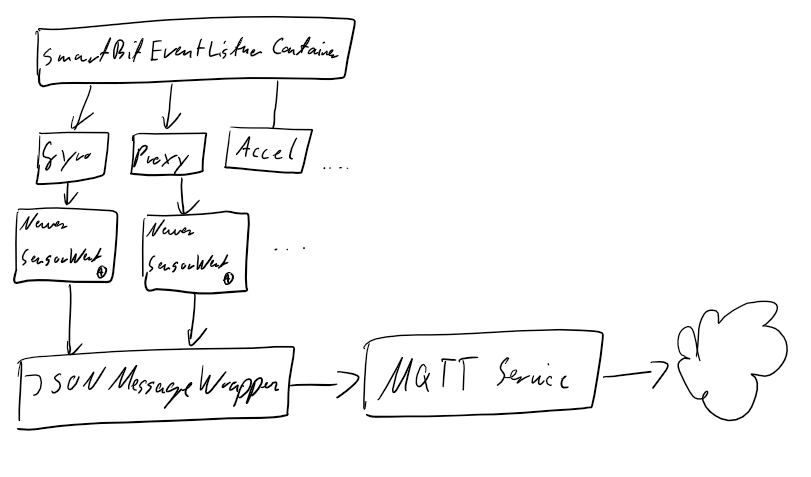
\includegraphics[width=.9\textwidth]{images/sensor_event_listener.png}
  \caption{Ablaufdiagramm SensorEventListener}
  \label{fig:sensor_event_listener}
\end{figure}
Die Klasse \textit{SmartBitEventListenerContainer} beeinhaltet SensorEventListener für alle Arten von untertstützten Sensoren.
Der Container dient lediglich der Datenhaltung.
Aufgabe der SensorEventListener ist es auf Sensorwert-Änderungen zu reagieren und eine entsprechende Callback-Funktion aufzurufen.
In dieser werden dann über statische Methoden der Klasse \textit{JSONMessageWrapper} update\_requests generiert und der gemessene Wert eingesetzt.
Die so generierte Nachricht wird anschließend über den gebundenen MQTT-Service an das vorher definierte Topic versendet.
\\\\
Die Anwendung ist nun betriebsbereit und beginnt bereits erste Nachrichten an die Kontrollanwendung zu senden.
Übermittelt werden die Sensordaten an den Broker mit einer QOS-Stufe von 0.
Verluste von update\_requests sind unproblematisch, da es je nach Taktung sehr schnell neue Sensorwerte gibt die übertragen werden können.
Eine exakte Zustellung ist hier nicht notwendig und verlangsamt eher den Übertragungsprozess.

\section{Sensoren}
Smartphones beeinhalten verschiedene Sensoren die Daten über die Umgebung erfassen können.
In der Android Anwendung werden folgende Sensortypen verwendet:
\begin{itemize}
  \item Lineare Beschleunigungssensoren
  \item Mikrofon
  \item Annäherungssensor
  \item Gyroskop
\end{itemize}

Beschleunigungs- bzw. Lagesensoren messen die Beschleunigung in $m/s^2$ für die drei Bewegungsrichtungen: X-, Y- und Z-Achse in einem festgelegten Zeitraum.
Eine Übersicht über die Anordungen der drei Axen ist in Abbildung \ref{fig:and_axes} zu sehen.
\begin{figure}[htbp]
  \centering
  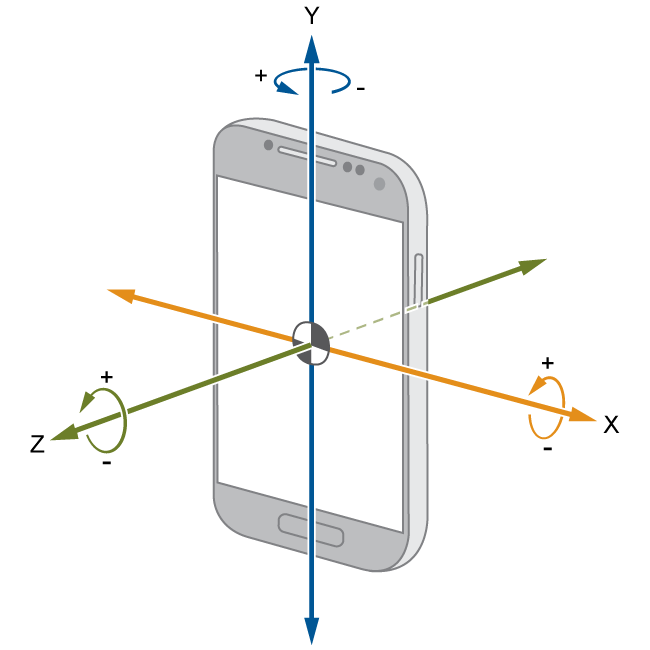
\includegraphics[width=.7\textwidth]{images/android_axes.png}
  \caption{Android-Koordinatensystem}
  \label{fig:and_axes}
\end{figure}
Die X-Achse verläuft horizontal durch das Display des Smartphones hindruch, die Y-Achse vertikal und die Z-Achse durchschneidet das Smartphone in die Tiefe.
\\\\
Die Frequenz mit der Messwerte erstellt werden kann manuell angegeben werden.
Hierfür stehen vier Schnelligkeitsstufen bereit.
\begin{table}[htbp]
  \centering
  \begin{tabular}{|c|p{4cm}|}
      \hline
      \textbf{Bezeichnung} & \textbf{Verzögerung} \\
	  \hline
      SENSOR\_DELAY\_FASTEST & Keine. Verwendet die Frequenz des Sensors.\\
      \hline
      SENSOR\_DELAY\_GAME & 20 ms\\
      \hline
      SENSOR\_DELAY\_UI & 60 ms\\
      \hline
      SENSOR\_DELAY\_NORMAL & 200 ms\\
      \hline
  \end{tabular}
  \caption{Sensor-Taktgeschwindigkeiten\cite{sensor-takt}}
  \label{tab:sensor_speeds}
\end{table}
Die mit der jeweiligen Frequenz aufgenommenen Beschleunigungssensordaten beeinhalten jedoch auch die Ergbeschleunigung.
Diese muss für die bereinigten, realen Werte zuerst noch von den aufgenommenen Werten subtrahiert werden\cite{accel_g}.
\section{Angaben für die Nachrichtenformate}
Alle Sensordaten besitzen ein festgelegtes Kürzel zur Standardisierung des Nachrichtenverkehrs.
Sie dienen vor allem der Adressierung der jeweiligen Daten in der Middleware und in der Library.
\\
Die Sensortyp Kürzel sind in Tabelle \ref{tab:sensor_types} zu finden. 
\begin{table}[htbp]
  \centering
  \begin{tabular}{|c|c|}
      \hline
      \textbf{TYPE-Kürzel} & \textbf{Beschreibung} \\
      \hline
      accel\_xyz & Lagesensor für die X, Y oder Z-Richtung \\
      \hline
       gyro\_xyz & Gyroskopsensor für die X, Y oder Z-Richtung \\
      \hline
      prox & Näherungssensor \\
      \hline
  \end{tabular}
  \caption{Sensor-Kürzel mit Beschreibung}
  \label{tab:sensor_types}
\end{table}

\section{Kommandos und Ausgaben}
Für die Ausgabe auf dem Smartphone sind verschiedene Kommandos definiert.
Diese sind der Tabelle \ref{tab:command_types} zu entnehmen.
\texttt{CMD-Kürzel} beschreibt die Notation des Kürzels mit dem eine Aktion ausgeführt werden kann.
Diese wird unter \texttt{Beschreibung} kurz zusammengefasst.
\texttt{return} gibt an, ob der Aufruf des Requests eine Antwort rücksendet und somit auch, ob ein Aufruf der Funktion in der Library blockiert oder nur sendet.

\chapter{Kontrollanwendung}\label{chap:server_software}

Für Vermittlung zwischen den Komponenten fungiert eine Server-Anwendung.
Sie ist in Python geschrieben und vermittelt zwischen UDP-Anfragen auf der einen Seite vom Client aus und MQTT-Anfragen vom Smartphone auf der anderen Seite.
User können über die Library RPC-Anfragen oder Sensor-Anfragen an den Server stellen.
Dies geschieht in form von JSON-Anfragen die per UDP übermittelt werden.
Der Server ist unter der localhost-Adresse 127.0.0.1 auf dem Port 5006 erreichbar.
Für die MQTT-Verbindung kommt dabei die unter OpenSource-Liznenz stehende MQTT-Library Paho der Eclipse-Foundation zum Einsatz. \cite{paho}


\section{Anforderungen}
Aus den Anforderungen ergeben sich folgende Aufgaben die der Server umsetzen muss:
\begin{itemize}
\item Sensoranfragen schnell beantworten
\item Anfragen die Funktionen auf dem Smartphone starte, müssen schnell an das Smartphone weitergereicht und gegebenfalls wieder beantwortet werden.
\end{itemize}
Damit Sensoranfragen schnell beantwortet werden können, werden die aktuellen Sensorworte fortlaufend vom Smartphone an den Server übermittelt.
Dieser speichert Sie dann, sobald ein Sensorwert gemessen und übermittelt wurde in eine interne, threadsichere Datenstruktur.
Hierdurch wird insbesondere der Latenzunterschied zwischen Smartphone und Localhost berücksichtigt.
UDP Anfragen per Localhost haben eine wesentlich geringe Latenz als MQTT-Anfragen, auf die das Smartphone reagieren muss.
Durch das Cachen auf dem Server liegen bei Anfragen per UDP, also von der Library aus, immer Sensordaten vor.

Um Funktionsanfragen zeitnah auszuführen müssen unterschiedliche Netzwerklatenzen berücksichtigt werden.
Die Übermittlung erfolgt asynchron zwischen Library und Smartphone, wobei zu erwarten ist dass Übermittlungen an das Smartphone mit einer höheren Latenz übertragen werden, als Anfragen zwischen Library und Server, da sich beide auf dem gleichen Host befinden.
Die Verbindung zwischen Library und Server erfolgt darüber hinaus über localhost und somit über ein Loopback-Device.
Loopback-Devices reichen Netzwerkpakete nicht herkömmlich über ein physisches Netzwerkinterface weiter sondern stellen ein virtuelles Gerät dar, dessen Übertragungsrate an die CPU gekoppelt ist.
Die Bandbreiten sind dadurch sehr hoch und die Latenzen gering.

Um die Latenzen und die damit verbundenen unterschiedlichen Auftrittszeitpunkte von Anfragen zu berücksichten, sowie eine möglichst effiziente Abarbeitung der selbiger zu ermöglichen wird eien paralelle Algorithmusstruktur verwendet.

\section{Interner Aufbau}
Die Serveranwendung mit dem Namen server.py ist aufgeteilt in einen Datenverwaltungsteil, DataHandler, und eine MQTT Anbindung, MQTTHandlerThread.
Da die Sensorwerte des Smartphoens vorrätig gehalten werden, wird außerdem eine Datenklasse für diese, SensorDB, intern gehalten.
Eine Übersicht über die Komponenten ist Abbildung \ref{fig:serverUml} zu entnehmen.
\begin{figure}[htbp]
  \centering
  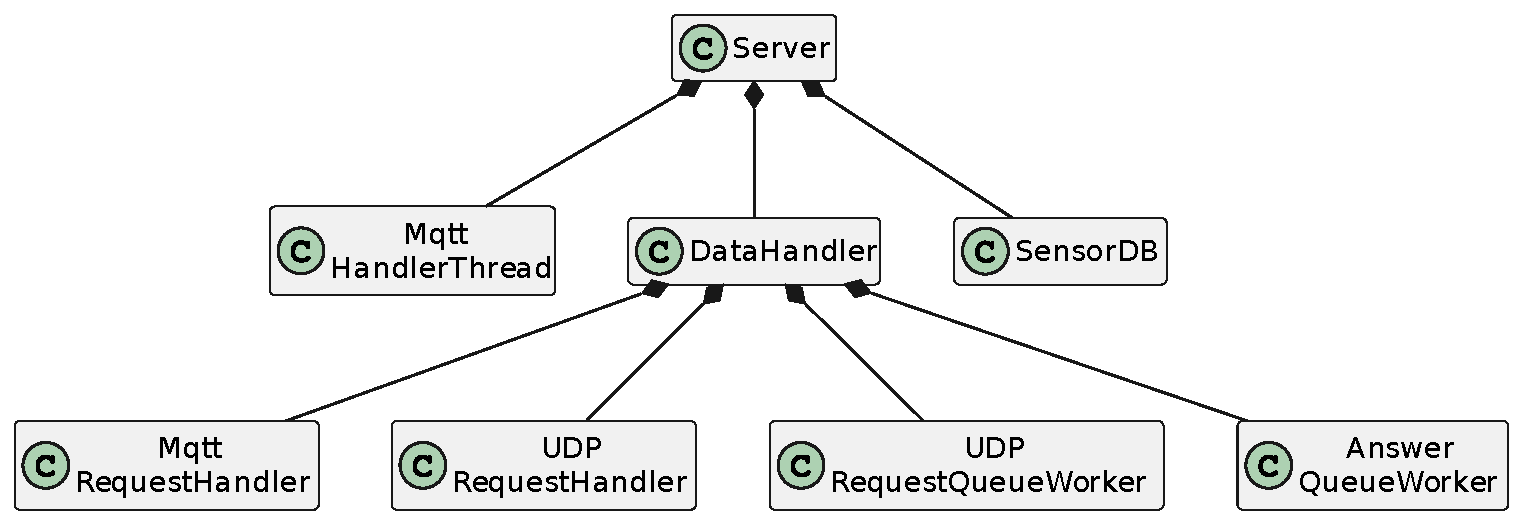
\includegraphics[width=\textwidth]{images/ServerUml}
  \caption{UML Digaramm Server}
  \label{fig:serverUml}
\end{figure}
DataHandler wiederrum teilt sich nochmal auf in vier seperate Funktionen, die als Threads nebenläufig laufen: MqttRequestHandler, UDPRequestHandler, UDPRequestQueueWorker und AnswerQueueWorker.

Die Funktionsweise und Zwecke dieser Threads wird im Folgenden an zwei Beispielen erläutert.
Für das erste Beispiel wird Abbildung \ref{fig:serverMqttReqPath} betrachtet.
Zu sehen ist ein MQTT-Request, also eine Anfragen des Smartphones, dass über MQTT an den Server gesendet wird.
Schnittstellen zu MQTT sind in der Abbildung grün, Schnittstellen zur Library per UDP, sind blau markiert.
\begin{figure}[htbp]
  \centering
  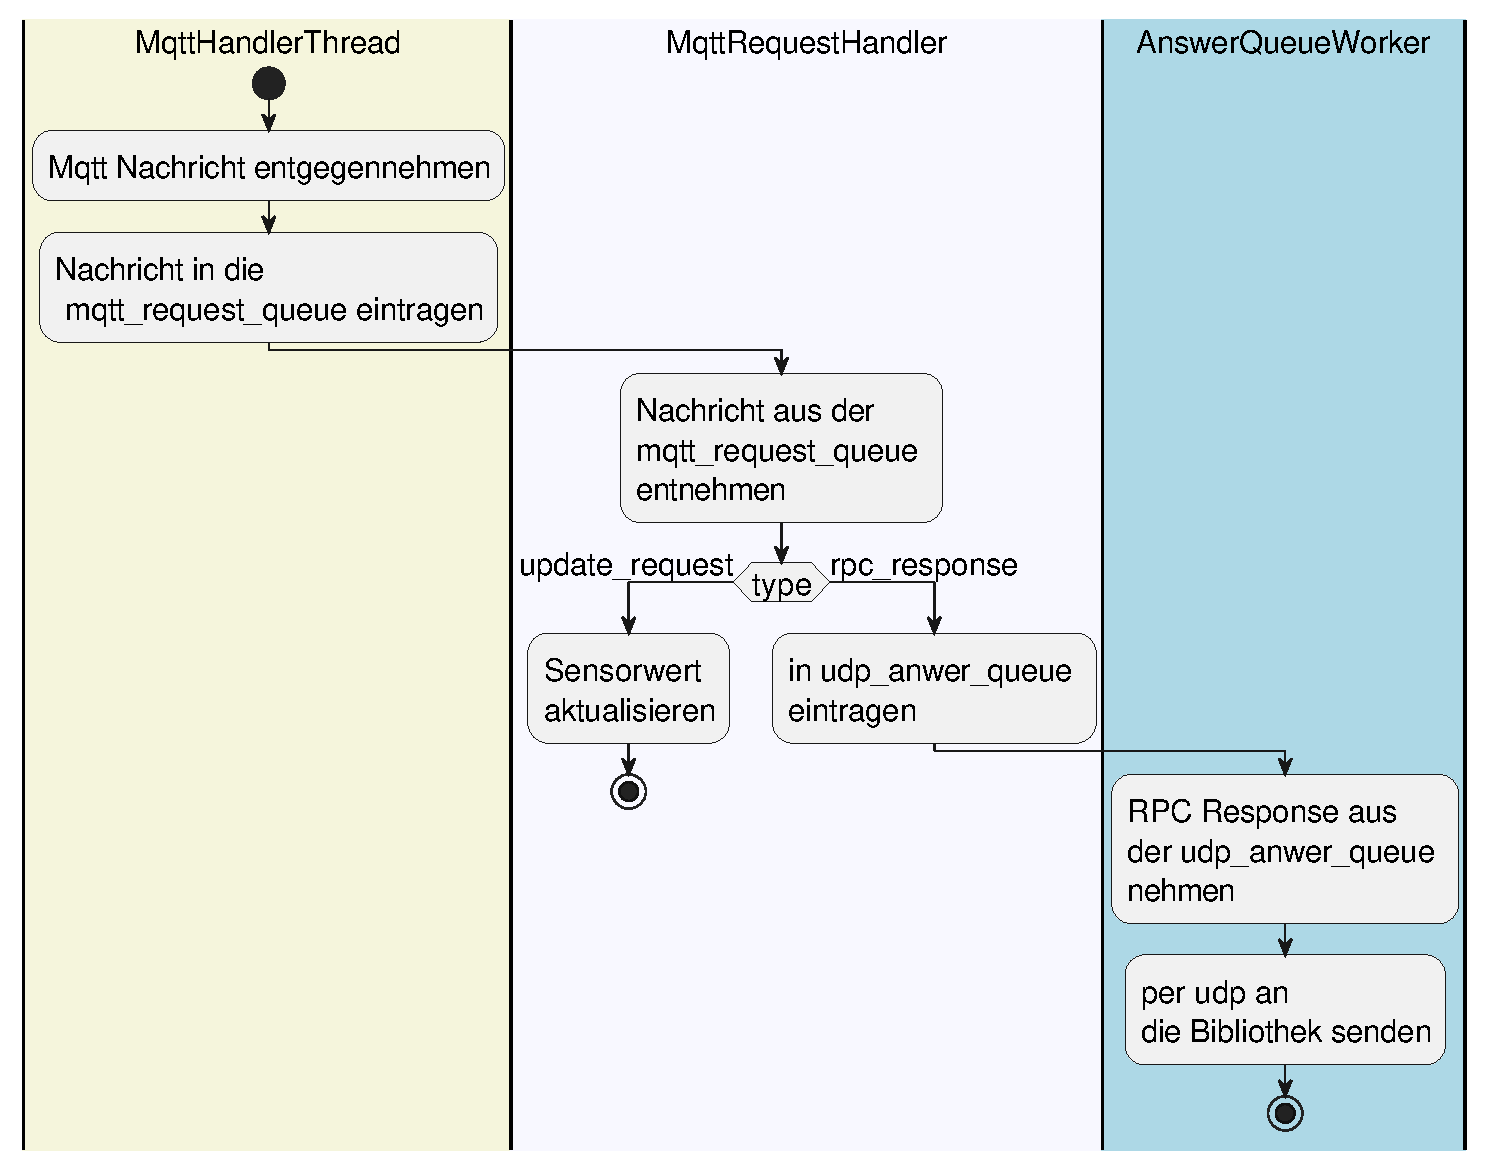
\includegraphics[width=\textwidth]{images/MqttRequestServerPath}
  \caption{Ablaufdiagramm MQTT Request}
  \label{fig:serverMqttReqPath}
\end{figure}
Erreicht ein MQTT Request den Server wird es im MQTTHandlerThread entgegengenommen.
Dieser setzt die Nachricht in eine MQTTRequestQueue ein.
Der MQTTRequestHandler des DataHandlers wartet bis ein Eintrag in der Queue vorhanden ist und nimmt gegebenenfalls eine Nachricht.
Daraufhin wird derTyp des Requests bestimmt.
Handelt sich um ein Sensorupdate muss nur der Sensorwert in der Datenbank aktualisiert werden.
Handelt es sich um eine rpc\_response, also um eine Antwort auf eine vorausgegangenes rpc\_request, dass einen Rückgabewert fordert, wird das request in eine udp\_answer\_queue eingefügt.
Der AnswerQueue Worker wartet, ähnlich wie der MQTT Request Handler, bis eine neue Nachricht vorhanden ist die per UDP an den Client gesendet werden soll und sendet diese dann gegebenfalls ab.

Das zweite Beispiel befasst sich mit dem Ablauf eines UDP-Requests, also einer Anfrage die mithilfe der Library gesendet wurde.
Der Ablauf ist in Abbildung \ref{fig:serverUDPReqPath} dargestellt.
Wie auch schon in der letzten Abbildung sind alle Schnittstellen zum Smartphone grün und alle Schnittstellen zur Library blau markiert.
\begin{figure}[htbp]
  \centering
  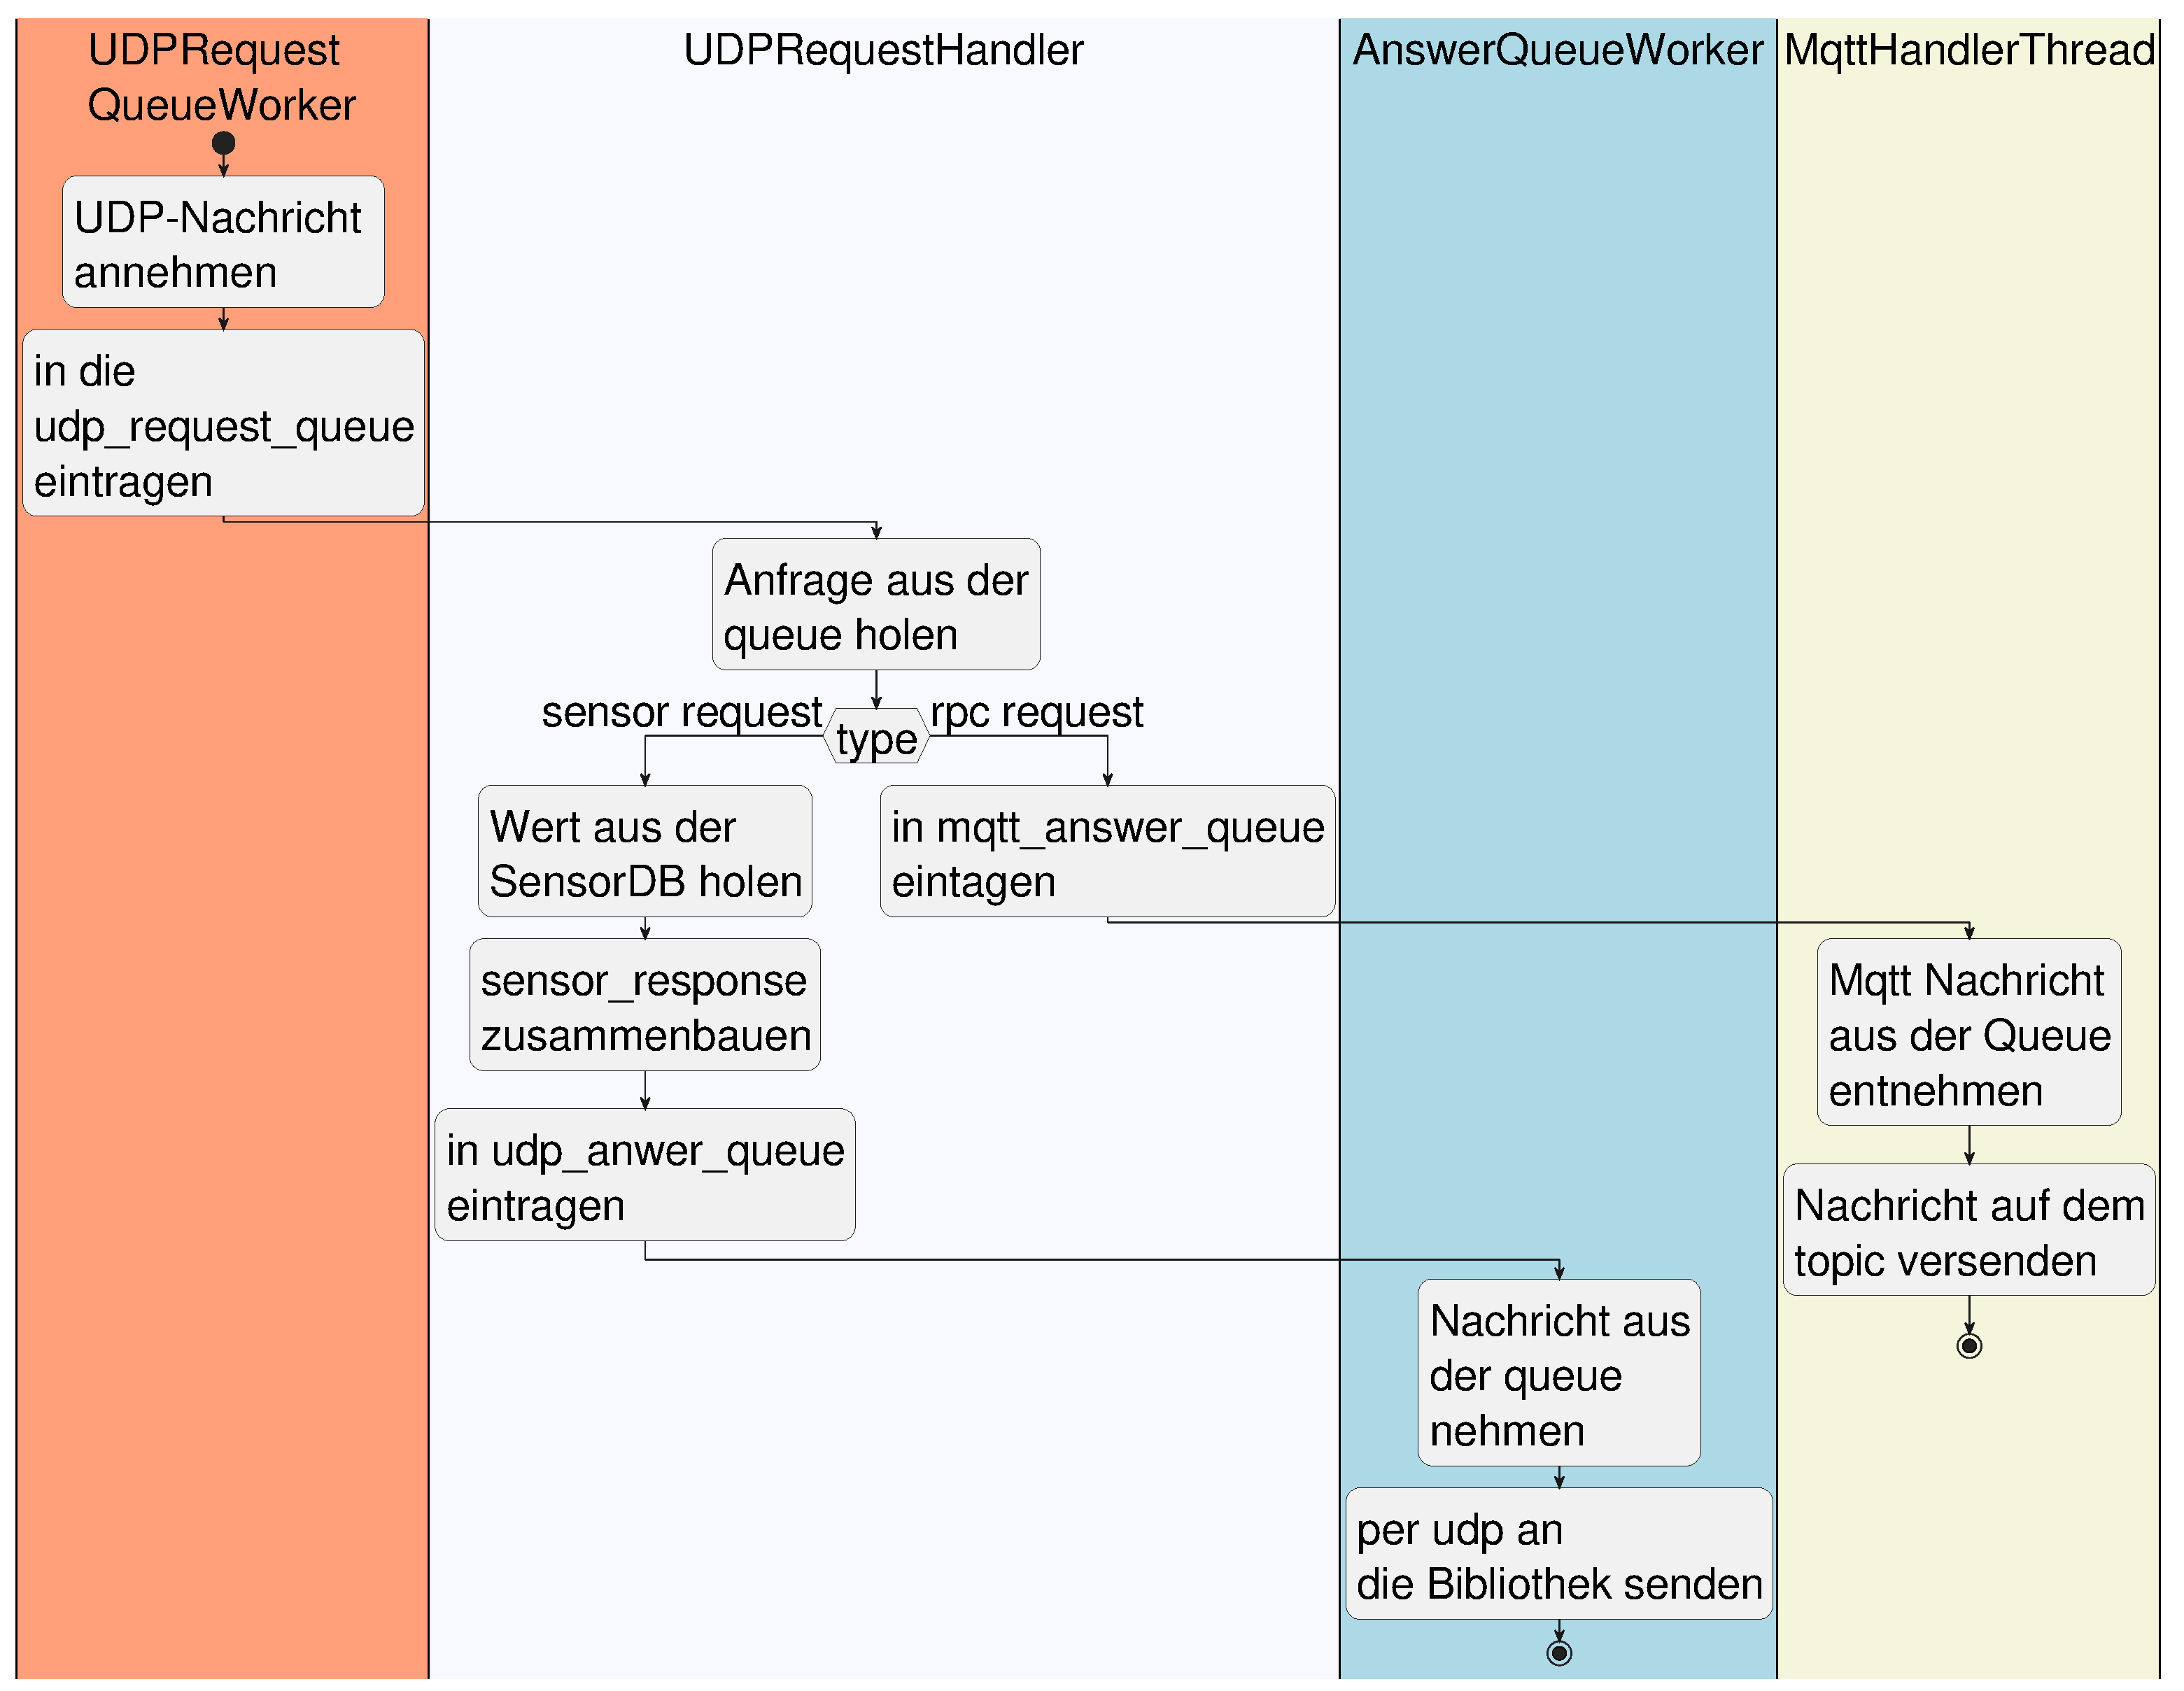
\includegraphics[width=\textwidth]{images/UDPRequestServerPath}
  \caption{Ablaufdiagramm UDP Request}
  \label{fig:serverUDPReqPath}
\end{figure}
Erreicht ein UDP Request den Server wird es vom UDPRequestQueue-Worker in eine UDP Request Queue gelegt.
Der UDPRequestHandler-Thread entnimmt die Nachricht und bestimmt den Anfragentyp.
Handelt es sich um eine Anfrage des Types RPC\_Request soll sie Aktionen auf dem Smartphone auslösen.
Sie muss an das Smartphone gesendet werden, was über MQTT möglich ist.
Dafür wird Sie ineine MqttAnswerQueue eingesetzt.
Der MQTTHandlerThread entnimmt Sie und sendet Sie per MQTT ab.
Ist Request hingegen ein SensorRequest, also eine Anfrage auf die ein Sensorwert geantwortet werden soll wird der nachgefragte Sensorwert über die Klasse SensorDB entnommen und in die Udp\_answer\_queue eingetragen.
Der AnswerQueueWorker entnimmt die Anfrage und sendet Sie per udp an die Library zurück.

Zusammenfassend erfüllen die Komponenten folgende Aufgaben.
Der MQTTHandlerThread nimmt Nachrichten direkt per MQTT an und gibt die Anfrage weiter.
Außerdem sendet er Nachrichten per MQTT, falls welche anfallen.
Der MQTTRequestHandler kümmert sich um das Verfahren von MQTT Requests.
Der UDPRequestQueue Worker nimmt wie der MQTTHandlerThread Anfragen die per UDP übermittelt wurden an und gibt Sie zur Behandlung entsprechend weiter.
Er sendet jedoch im Gegensatz keine Responses zurück.
Hierfür gibt es den AnswerQueueWorker, dessen einzige Aufgabe es ist Antworten per UDP zurück zu übermitteln.

Die Kommunikation zwischen den Threads funktioniert über synchronisierte Queues des queue-Moduls\cite{python_queue} der cpython Implementierung.
Es handelt sich um eine threadsichere Monitorklasse, die einen gleichzeitigen Zugriff zweier unterschiedlicher Threads durch Locks verhindert.

\chapter{Programmierumgebung}\label{chap:libs}
Die Bibliotheken bilden die Einstiegsstelle für Nutzer um die Anwendung fernzusteuern oder Sensorwerte abzufragen.
Funktionsaufrufe liegen jeweils in den Sprachen C, Java und Python vor.
Daten werden wie in Kapitel \ref{chap:architektur} in Abbildung \ref{fig:design} gezeigt per UDP an eine Serveranwendung gesendet.
Diese sendet die Daten dann nach gegebenenfalls per MQTT an das Smartphone weiter, oder wieder per UDP zurück.
Die Bibliotheken senden und empfangen alle jeweils Daten per UDP.
Hierfür werden Sockets benötigt.
Für's Empfangen muss der Socket binded sein.
Die Serveranwendung ist auf dem Port 5006 erreichbar.
Antworten erwarten die Bibliotheken auf dem Port 5005.

\chapter{Evaluation}\label{chap:eval}
In disem Kapitel wird die Verwendung des Frameworks anhand dem Beispiel \textit{Alarmanlage} vorgestellt.
Gezeigt wird, wie die Aufgabe in der Programmierumgebung gelöst wurde und wie sich die Aufgabe auf dem Smartphone äußert.
Dadurch wird überprüft, ob die Anforderungen an die Smartphone-Anwendung erfüllt wurden.
Neben Anforderungen Benutzung betreffen gibt es auch welche, die die Latenzen betreffen.
Transportwege müssen berücksichtigt werden.
Die Zeiten werden in drei verschiedenen Umgebungen überprüft: In nächster Nähe zum MQTT-Server, in mittlerer Nähe und in einer virtuellen Umgebung über ein simuliertes NAT-Netzwerk.

\section{Beispielverwendung}
Die Verwendung der Lösung wird anhand des \textit{Alarmanlage}-Beispiel vorgestellt.
In der Programmierumgebung wird dabei die Bibliothek in Python verwendet.

Damit Nachrichten ausgetauscht werden können muss zuerst das Kontrollprogramm gestartet werden.
Es wird mit dem Befehl \texttt{python ./server.py} in einer lokalen Shell gestartet.
Der Vorgang wird in Abbildung \ref{fig:start_controll_app} dargestellt.
Es handelt sich um das Python-Skript \textit{server.py}.
\begin{figure}[htbp]
  \centering
  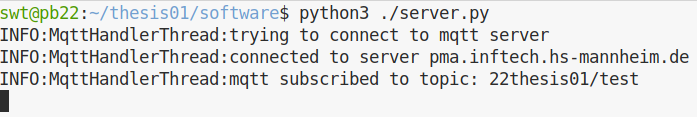
\includegraphics[width=.8\textwidth]{images/server_logging}
  \caption{Start der Kontrollanwendung}
  \label{fig:start_controll_app}
\end{figure}
Die Anwendung meldet, dass Sie sich erfolgreich mit dem MQTT-Broker verbunden und das korrekte Topic abboniert hat.
Die Kontrollanwendung loggt neben diesen Informationen auch rpc-requests und responses.
Sensor-requests und responses werden wegen ihrer hohen Anzahl nicht geloggt.

Die Implementierung der Lösung der Aufgabe ist in Listing \ref{lis:alarm} vorgestellt.

\lstset{language=python, captionpos=b, frame=single, numberstyle=\tiny, style=customcs}
\lstinputlisting[label=lis:alarm, caption=Alarmanlage-Beispiel]{listings/code_examples/alarm.py}
Die Bibliothek wird in Zeile 2 importiert.
Dafür muss die Datei \texttt{smartbit.py} im gleichen Ordner wie das Programm gespeichert sein.
In Zeile 4 wird ein Phone-Objekt erstellt, über das Sensor-Auslesemethoden wie \texttt{get\_x\_accel()} oder Smartphone-Ausgaben wie \texttt{vibrate()} augerufen werden können.
Da das Programm nie abbrechen soll, außer wenn es in der shell gestoppt wird, wird in einer While-True Schleife der Näherungssensor immer wieder abgefragt.
Anschließend wird eine halbe Sekunde gewartet um den Server nicht mit Anfragen zu überlasten.
Ist der abgerfragte Näherungssensorwert wie in der achten Zeile überprüft wird 0.0, dann liegt eine Näherung vor.
Auf dem Smartphone wird dann mit der  Methode \texttt{write\_text()} der Text ALARM usgegeben.
Das Smartphone vibriert 5 mal hintereinander im Abstand von 200 ms für eine Sekunde und lässt die Signal-LED blinken.
Insgesamt werden die RPC-Funktionen vibrate, toggle\_button und write\_text aufgerufen.
Keine dieser Funktionen liefert einen Rückgabewert.

Die Bibliothek sendet die Nachrichten an das Smartphone.
Nähert sich eine Person dem Smartphone wird der Code in der If-Bedingung ausgeführt.
Die jeweiligen Nachrichten werden als rpc\_request per UDP an die Kontrollanwendung gesendet.
Dort werden Sie angenommen, geloggt und per MQTT an das Smartphone weitergereicht.
Eine Übersicht der gesendeten Nachrichten ist in Abbildung \ref{fig:req_controll_app} zu sehen.
\begin{figure}[htbp]
  \centering
  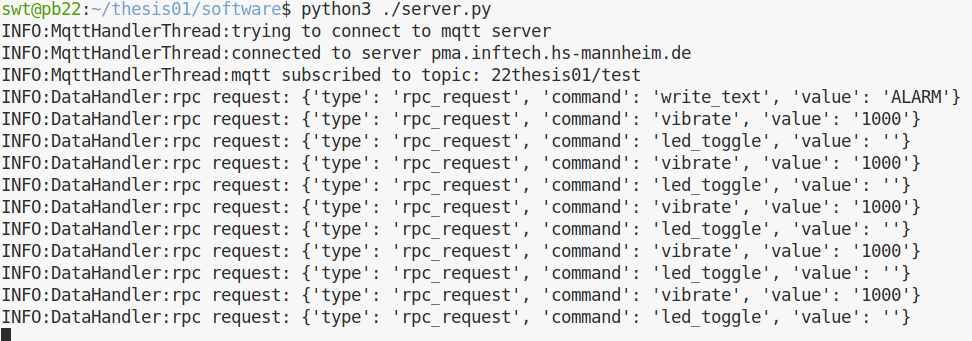
\includegraphics[width=\textwidth]{images/server_requests}
  \caption{Nachrichtenversand der Kontrollanwendung}
  \label{fig:req_controll_app}
\end{figure}
Die Nachrichten werden im JSON Format übertragen.
rpc\_requests haben ein Typ-Feld, ein Kommando und einen Paramterwert für das Kommando.
Write\_text ist für Textausgaben auf dem Smartphone, vibrate um das Smartphone vibrieren zu lassen und led\_toggle um die LED anzusprechen.
Für write\_text wird der gibt der Parameter-Wert den anzuzeigenden Text an.
Vibrate erwartet für value die Zeitdauer der vibrierung in ms.
led\_toggle erwartet keinen Parameterwert, da der gesamte Aufruf lediglich die Farbe der LED wechselt.
Es ist nicht vorgesehen, dass die Farbe manuell gesetzt werden kann.

Auf dem Smartphone ist die App zu Anfang im Initialmodus.
Dieser ist in Abbildung \ref{fig:initial_app} dargestellt.
\begin{figure}[htbp]
  \centering
  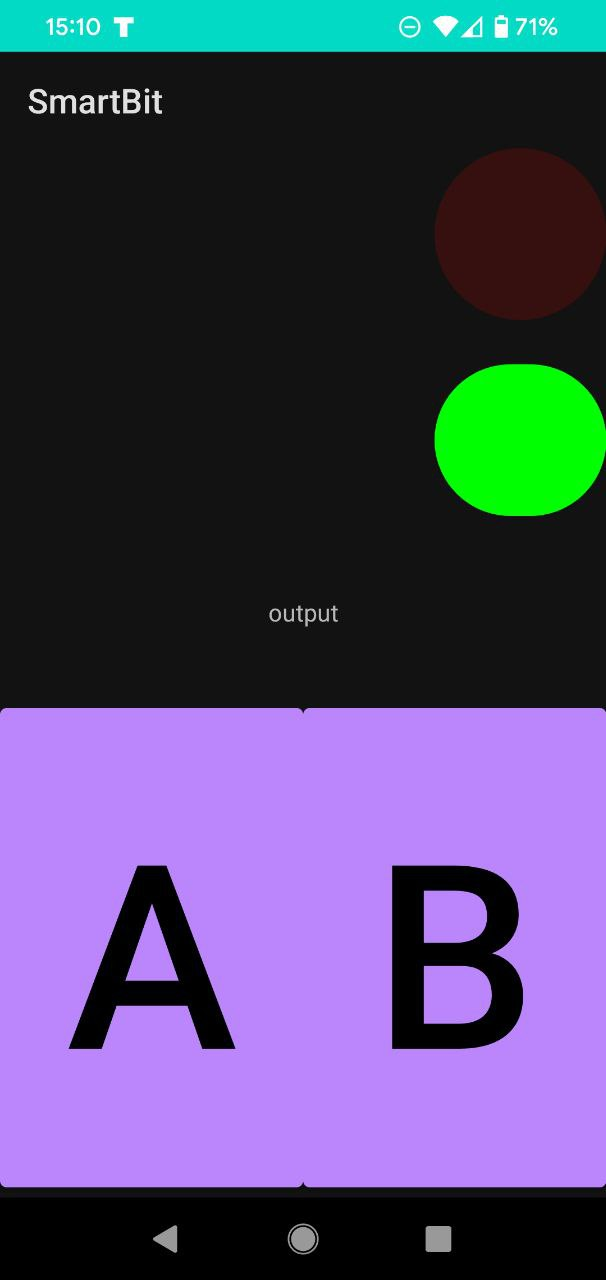
\includegraphics[height=0.4\textheight]{images/app_initial}
  \caption{Initialzustand der Anwendung}
  \label{fig:initial_app}
\end{figure}
Zu sehen sind zwei Buttons, beschriftet mit A und B.
Das textfeld liegt in der Mitte und zeigt zum Start den Text \textit{output} an.
Daneben gibt es noch eine Vorgangs-LED die ausgegraut oben rechts über der Signal-LED liegt.
Sie leuchtet, wenn gerade ein Vorgang wie das Ausführen einer Vibration auf dem Smartphone ausgeführt wird.

Nähert man sich dem Smartphone geht es über in den Alarmzustand der in Abbildung \ref{fig:app_alarm} dargestellt ist.
\begin{figure}[htbp]
  \centering
  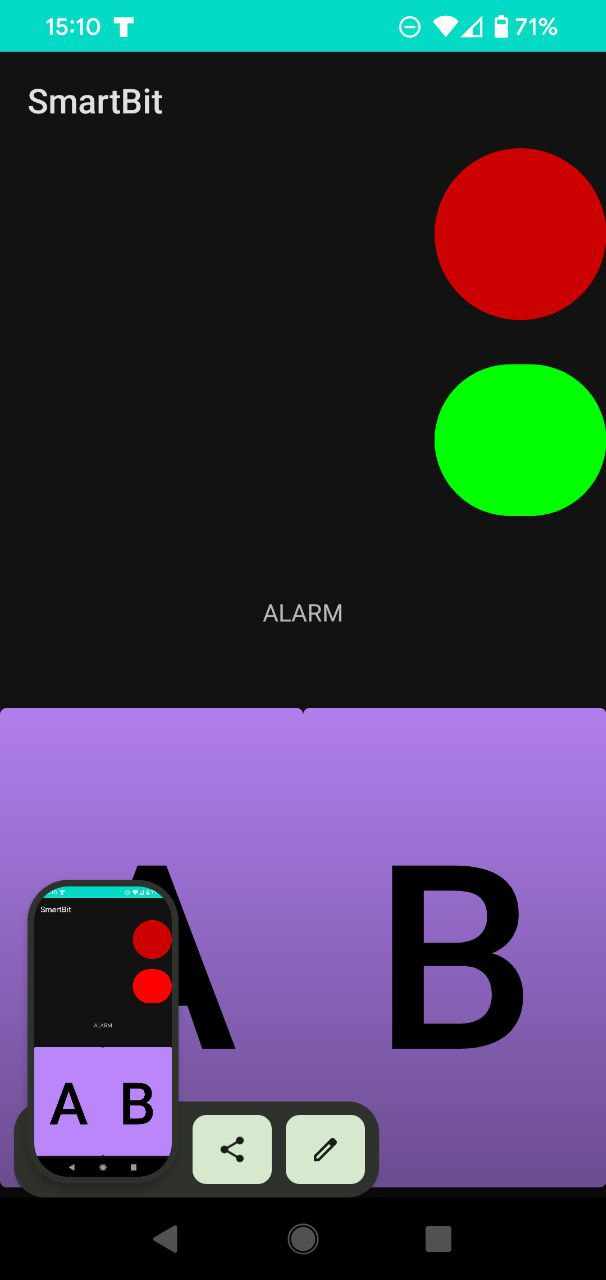
\includegraphics[height=0.4\textheight]{images/app_alarm}
  \caption{Initialzustand der Anwendung}
  \label{fig:app_alarm}
\end{figure}
Erkennbar ist, dass das Textfeld den Wert \textit{ALARM} darstellt.
Die Farbe der LED hat sich von grün auf rot und wieder auf grün geändert.
Das ist erkennbar an der kleinen Screenshot-Vorschau links unten die unmittelbar vor dem in der Abbildung zu sehenden Screenshot zu sehen ist.
Die Vorgangs-LED leuchtet tief rot um zu signalisieren dass gerade eine Ausgabe ausgeführt wird.
Nicht sichtbar ist das haptische vibrationsfeedback.
Hierfür dient jedoch die Vorgangs-LED.
Sie ist auch hilfreich um bei Smartphones mit sanften Vibrationsausgaben eine Ausgabe zu erkennen.

Die Reaktionszeit liegt unter einer Sekunde.
Die Ausgabe erscheint als direkter Grund der Annäherung.

\section{Messergebnisse}
Damit die Benutzbarkeit sichergestellt ist, müssen Latenzzeiten zwischen Smartphone und Programmierumgebung in einem akzeptablen Rahmen liegen.
Um dies herauszufinden werden die Latenzzeiten gemessen.
In diesem Kapitel wird die Latenzzeit von drei Standorten aus gemessen.

Der erste Einsatzort ist im gleichen Netzbereich wie der MQTT-Broker wodurch die Transferstrecke reduziert wird.
Neben der Latenzzeit zum Broker ist jedoch auch die Anzahl der angemeldeten Geräte am gleichen AccessPoint interessant.
Da die Geräte in direktem Wettbewerb um Sendezeit stehen bedeuten mehr Geräte an einem AccessPoint größere Latenzen.
In den Messungen werden nur WLAN-Verbindungen nach dem Standard WLAN 802.11n berücksichtigt.
Es sind dabei stets beide Geräte, Lokaler PC und Smartphone per WLAN mit dem Internet verbunden.
Untersucht wird lediglich die Zeitspanne zwischen rpc\_request und rpc\_response.
Sensor\_requests kommunizieren stets per loopback-interface mit der Kontrollanwendung.
Daher die Latenzzeiten gering.
Im Durchschnitt belaufen Sie sich auf unter 1ms.
Die Messungen sind  für den Fall interessant, für den Studierende an der Hochschule die Lösung nutzen möchten.
Zum Beispiel in Laboren.

Der zweite Einsatzort ist ein Heimnetz, das etwa 8 Hops entfernt vom MQTT-Broker liegt.
Etwa 8 Geräte sind dabei auf dem Access Point angemeldet.
Die Messergebnisse sind relevant für die Heimarbeit oder das Erledigen von Hausaufgaben.
Die Ergebnisse sind in Abbildung \ref{fig:measure_home} dargestellt.
\begin{figure}[htbp]
  \centering
  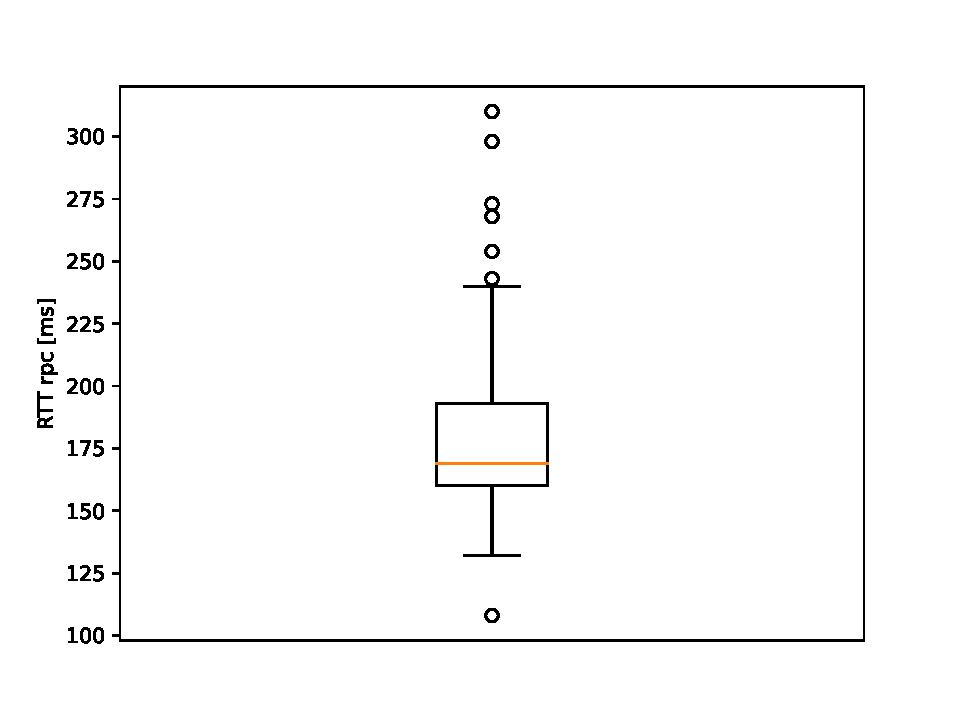
\includegraphics[width=0.6\textwidth]{images/timing_at_home}
  \caption{Zeitmessungen im Heimnetz}
  \label{fig:measure_home}
\end{figure}
Insgesamt wurden 100 Messungen durchgeführt.
Im Mittel beträgt die Reaktionszeit 537 ms.
Die Streuung ist bei einer Standardabweichung von 238ms allerdings auch sehr breit gestreut.
Alle Messungen blieben jedoch unter 1s Reaktionszeit.

Der letzte Einsatzort ist in einer virtuellen Maschine auf dem lokalen PC das über den virtuellen Netzwerkkontroller aus einem NAT-Netzbereich auf das Internet zugreift.
Das Smartphone befindet sich direkt im Netzbereich des lokalen PCs.
Die gemessenen Daten sind in Abbildung \ref{fig:measure_vm} dargestellt.
\begin{figure}[htbp]
  \centering
  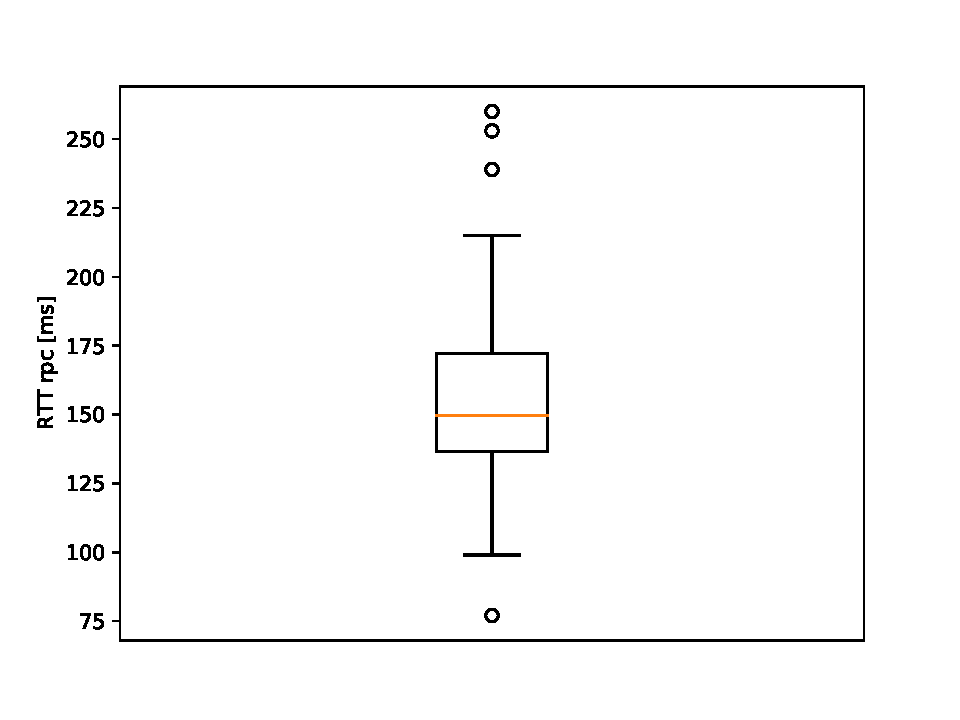
\includegraphics[width=0.6\textwidth]{images/timing_vm}
  \caption{Zeitmessungen in der virtuellen Maschine}
  \label{fig:measure_vm}
\end{figure}
Wieder wurden 100 Messungen vorgenommen.
Im Mittel beträgt die Reaktionszeit nun 3255 ms.
Die Streuung ist mit einer Standardabweichung von 845 ms relativ gleichgroß.
Die Reaktionszeit ist also im Durchschnitt sehr hoch, etwa sechs mal langsamer als bei einer Verwendung der Programmierumgebung auf dem Hostsystem.
Eine direkte Assoziation zwischen Eingabe und Ausgabe kann nicht garantiert werden.

\chapter{Fazit}\label{chap:fazit}
Die implementierte Lösung erfüllt die gestellten Anforderungen zum größten Teil zufriedenstellend.
Latenzprobleme per MQTT treten nicht auf.
Trotz einem QOS-Level 0 werden auch Ausgabeanfragen sicher übertragen und ausgeführt.
Da die Nachrichten über TLS übertragen werden ist der Austausch sicher.
Logging-Möglichkeiten in der Kontrollanwendung und der Android-App erleichterten die Entwicklung sehr und halfen bei der Fehlersuche.
Neben den Vorteilen wurden jedoch während der Konzeption einige Fehlentscheidungen getroffen.
Es ist nicht möglich den gleichen Programmcode auf mehreren Smartphones auszuführen, da die Kontrollanwendung die Sensordaten nicht pro Gerät unterscheidet.
Eine Kontrollanwendung speichert immern nur die Sensordaten eines Smartphones.
Außerdem ist es nicht nur nicht möglich ein Programm an mehrere Smartphones zu koppeln, sondern es ist auch unmöglich mehrere Kontrollanwendungen generell zu betreiben.
Diese würden alle auf dem gleichen Topic senden.
Ausgabeanfragen würden von allen Smartphones ausgeführt werden.
Sensorwerte anderer Smartphones würden die richtigen überschreiben.
Es können also keine Gruppen- und nicht mehr als eine Einzel-Session erstellt werden.
Für den Laborbetrieb ist die Lösung so nicht geeignet.
Letzteres Problem lässt sich einfach umgehen, indem man vor dem Start der Kontrollanwendung in der Konfigurationsdatei ein anderes Topic angibt.
Damit das Smartphone auch auf dem gleichen Topic kommuniziert müsste man es ebenfalls abändern können, denn die Smartphone-Konfigurationsdatei kann nur in der Entwicklungsumgebung geändert werden.
Das bedeutet einen erheblichen Mehraufwand.
Share-Preferences könnten hierbei eingesetzt werden, damit das Topic im Nachhinein App-Seitig nochgeädert werden kann.
So könnten immerhin insgesamt mehrere Smartphones insgesamt genutzt werden.
Eine weitere Fehlentscheidung bestand in der Auswahl von JSON als Kommunikationsstandard zwischen Middleware und Programmierumgebung.
Sowohl für Java, als auch für C sind zusätzliche JSON-Parser nötig.
Für C muss dieser vor dem Kompilierprozess hinzugefügt werden.
Unter Linux kann die Abhängigkeit einfach nachinstalliert und als Option mit angegeben werden.
Auf Windows-PCs ist dies jedoch etwas aufwändiger.
Ein Binärprotokoll würde Abhilfe schaffen.
Der Parser müsste selbst implementiert werden, allerdings nur einmal in der Kontrollanwendung.
Dadurch würde auch die Nachrichtengröße sinken.
Zwischen Middleware und Android-App könnte weiterhin JSON eingesetzt werden, da beide integrierte JSON-Parser besitzen.
Die Standardadisierung über eine JSON-Datei, die die Vorlagen für alle Nachrichten beinhaltet erhöht zwar die Übersicht bei vielen Nachrichtenformaten und bietet Raum für eventuelle Erweiterungen, stand der Entwicklung jedoch häufig im Weg.
Die Nachrichtenformate besitzen meist zu wenig Felder, als dass eine Standardisierung Sinn ergäbe.
So endete Sie meistens in zusätzlichem, unübersichtlichem Code.
Ein weiterer Nachteil liegt in der Speicherung von Sensorwerten.
Es wird immer nur der aktuelle Sensorwert in der Kontrollanwendung gehalten, bis der nächste kommt.
Eingeführt wurde er, damit sich Latenzen nicht so stark äußern und der Sensorwert trotzdem abgefragt werden kann.
Er hat jedoch kein Ablaufdatum.
Bei einem Verbindungsabbruch seitens des Smartphones wird weiterhin der zuletzt verfügbare Wert eingetragen.
Erhöhen sich die Latenzen kann nur ein einzelner Wert abgefragt werden.
Ein größerer Pufferspeicher mit einer festen Größe und Ablaufdatum wäre optimal.
So könnten bei erhöhten Latenzen trotzdem weiter valide, echte Sensorwerte zurückgegeben werden anstatt Kopien des zuletzt gespeicherten.
Durch ein Ablaufdatum könnte man eine Maximalzeit festlegen in der die Sensorwerte valide wären.

Kombinierbar wäre dies mit einem Stapel-Versand von Sensorwerten.
Smartphone App könnten sich in in periodischen Zeitabständen Nachrichten zur Latenzmessung senden.
Sollte sich diese erhöhen könnten Sie umschallten in einen Stapel-Übertragungsmodus in dem statt immer nur einem Sensorwert gleich mehrere übertragen werden.
JSON unterstützt diese Übermittlung mit der Array-Schreibweise.
So könnte die Bandbreite besser ausgenutzt werden und Latenzen umgangen.
Denkbar wäre außerdem Sensorwerte überhaupt erst nach Sendeaufforderung vom Smartphone an die Kontrollanwendung zu versenden.
Während die Android-App auf dem Smartphone läuft werden kontinuierlich von allen Sensoren die Sensorwerte übertragen.
Ein erhöhter Energieverbrauch ist die Folge.
Wünschenswert wäre spezifizieren zu können welche Ausgabemöglichkeiten auf dem Display angezeigt werden sollen.
Insbesondere falls durch eine Weiterentwicklung neue Ausgabemöglichkeiten dazukommen.
Dies könnte ähnlich wie bei der Platzierung von Widgets auf dem Homescreen gelöst werden.
Ausgabeelemente könnten aus einer Art Baukasten an die gewünschte Position gezogen werden, wo Sie dann verwendet werden können.
So könnte der Platz auf dem Bildschirm besser genutzt werden.

% Listen wenn überhaupt ans Ende und nicht an den Anfang.
% Meist ist das aber unnötig.
% \listoffigures % Liste der Abbildungen 
% \listoftables % Liste der Tabellen
\newpage

\bibliographystyle{plain} % Literaturverzeichnis
\begin{btSect}{thesis} % mit bibtopic Quellen trennen
\addcontentsline{toc}{chapter}{Literaturverzeichnis und Online-Quellen}
\section*{Literaturverzeichnis}
\btPrintCited
\end{btSect}
\begin{btSect}{online}
\section*{Online-Quellen}
\btPrintCited
%\bibliography{online}
\end{btSect}
% dann mit "bibtex thesis1" und "bibtex thesis2" arbeiten

\end{document}
;;; Local Variables:
;;; ispell-local-dictionary: "de_DE-neu"
;;; End:


